\begin{filecontents*}[overwrite]{run_all.py}
# %% Setup and reproducibility
from pathlib import Path
import sys, platform, time, json, math
import numpy as np
import matplotlib
matplotlib.use('Agg')
import matplotlib.pyplot as plt
from scipy.special import expit, ndtr, ndtri
OUT = Path(__file__).resolve().parents[1] / 'outputs'; OUT.mkdir(exist_ok=True)
plt.rcParams.update({'font.size':10, 'axes.grid':True, 'grid.alpha':.25,
                     'figure.dpi':160, 'savefig.dpi':250, 'savefig.bbox':'tight'})
SEED=20260916
M_GBM=65536; M_SV=32768; BATCH=1024
RESULTS={'seed':SEED, 'python':sys.version.split()[0], 'numpy':np.__version__,
         'platform':platform.platform(), 'M_GBM':M_GBM,'M_SV':M_SV}
def summary(x):
    x=np.asarray(x); m=float(x.mean()); se=float(x.std(ddof=1)/np.sqrt(x.size))
    return {'mean':m,'se':se,'lo':m-1.96*se,'hi':m+1.96*se}
def slope_ci(batch_errors, hs, seed=17):
    # Resample independent path batches; retain dependence across levels.
    a=np.asarray(batch_errors); hs=np.asarray(hs)
    fit=lambda v: np.polyfit(np.log(hs),np.log(v),1)[0]
    rng=np.random.default_rng(seed)
    slopes=[fit(a[rng.integers(len(a),size=len(a))].mean(axis=0)) for _ in range(500)]
    return [float(fit(a.mean(axis=0))), *np.quantile(slopes,[.025,.975]).tolist()]
def savefig(name):
    plt.tight_layout(); plt.savefig(OUT/(name+'.png')); plt.savefig(OUT/(name+'.pdf'))
    show_figure(plt.gcf()) if 'show_figure' in globals() else None
    plt.close()
def gbm(dW,h,method,mu=.2,sigma=.3,s0=100.):
    # Rows are time, columns independent paths; no Python loop over paths.
    if method=='exact': return s0*np.exp((mu-.5*sigma*sigma)*dW.shape[0]*h+sigma*dW.sum(axis=0))
    f=1+mu*h+sigma*dW
    if method=='Milstein': f=f+.5*sigma*sigma*(dW*dW-h)
    return s0*np.prod(f,axis=0)
def sv(d1,d2,h,mu=.05,kappa=2.,theta=-.2,xi=.6, balanced=False):
    x=np.full(d1.shape[1],np.log(100.)); y=np.zeros_like(x)
    decay=np.exp(-kappa*h)
    noise=xi*np.sqrt(-np.expm1(-2*kappa*h)/(2*kappa*h))
    for a,b in zip(d1,d2):
        g=.1+.4*expit(y)
        x += (mu-.5*g*g)*h+g*a
        if balanced:
            y=theta+decay*(y-theta)+noise*np.sqrt(1+y*y)*b
        else:
            y += kappa*(theta-y)*h+xi*np.sqrt(1+y*y)*b
        assert np.all(np.isfinite(y)) and np.all(np.abs(x)<700)
    s=np.exp(x)
    assert np.all(np.isfinite(s)) and np.all(s>0) and np.all(np.isfinite(y))
    return s,y
print('Reproducibility:', RESULTS)
# %% GBM: nested paths, strong and weak errors
ng=np.array([4,8,16,32,64,128,256,512,1024]); hg=1/ng
rng=np.random.default_rng(np.random.SeedSequence([SEED,1]))
gerr={k:[] for k in ['EM','Milstein']}; gdiff={k:[] for k in gerr}
gterm={k:[] for k in ['exact','EM','Milstein']}; batches={k:[] for k in gerr}
start=time.perf_counter()
for b in range(M_GBM//BATCH):
    fine=rng.normal(size=(ng[-1],BATCH))*np.sqrt(hg[-1]); exact=gbm(fine,hg[-1],'exact')
    errors={k:[] for k in gerr}; diffs={k:[] for k in gerr}
    for n,h in zip(ng,hg):
        dw=fine.reshape(n,ng[-1]//n,BATCH).sum(axis=1)
        for method in gerr:
            s=gbm(dw,h,method); errors[method].append(abs(s-exact)); diffs[method].append(s-exact)
            if n==32: gterm[method].append(s)
    gterm['exact'].append(exact)
    for method in gerr:
        gerr[method].append(np.array(errors[method])); gdiff[method].append(np.array(diffs[method]))
        batches[method].append(np.array(errors[method]).mean(axis=1))
G={}; analytic_mean=100*np.exp(.2); analytic_var=10000*np.exp(.4)*np.expm1(.09)
for method in gerr:
    gerr[method]=np.concatenate(gerr[method],axis=1); gdiff[method]=np.concatenate(gdiff[method],axis=1)
    G[method]={'strong':[summary(v) for v in gerr[method]],'weak_signed':[summary(v) for v in gdiff[method]],
               'slope':slope_ci(np.array(batches[method])[:,2:],hg[2:])}
for k in gterm: gterm[k]=np.concatenate(gterm[k])
bias_exact=100*np.exp(ng*np.log1p(.2/ng))-analytic_mean
G.update({'n':ng.tolist(),'analytic_mean':analytic_mean,'analytic_variance':analytic_var,
          'exact_mean_check':summary(gterm['exact']), 'exact_sample_variance':float(gterm['exact'].var(ddof=1)),
          'analytic_bias':bias_exact.tolist(),'elapsed_seconds':time.perf_counter()-start})
G['variance_check']=summary((gterm['exact']-analytic_mean)**2)
for method in ['EM','Milstein']:
    k=7 if method=='EM' else 9
    wb=-gdiff[method].reshape(9,M_GBM//BATCH,BATCH).mean(axis=2).T[:,:k]
    G[method]['weak_slope']=slope_ci(wb,hg[:k])
G['analytic_weak_slope']=float(np.polyfit(np.log(hg),np.log(abs(bias_exact)),1)[0])
for method in ['EM','Milstein']:
    print(method,'strong slope, bootstrap 95% CI:',G[method]['slope'])
    print('Weak slope and bootstrap CI:',G[method]['weak_slope'])
    print(' n     strong L1 (SE)        signed weak bias (SE)      analytic bias')
    for j,n in enumerate(ng):
        a=G[method]['strong'][j]; d=G[method]['weak_signed'][j]
        print(f'{n:4}  {a["mean"]:.6f} ({a["se"]:.6f})  {d["mean"]:+.6f} ({d["se"]:.6f})  {bias_exact[j]:+.6f}')
print('Exact-law moments:', {k:G[k] for k in ['analytic_mean','analytic_variance','exact_mean_check','exact_sample_variance']})
fig,ax=plt.subplots(1,2,figsize=(10,4))
for method in ['EM','Milstein']:
    ss=G[method]['strong']; ww=G[method]['weak_signed']
    ax[0].errorbar(hg,[v['mean'] for v in ss],yerr=[1.96*v['se'] for v in ss],marker='o',label=method)
    ax[1].errorbar(hg,-np.array([v['mean'] for v in ww]),yerr=[1.96*v['se'] for v in ww],marker='o',label=method)
ax[1].plot(hg,-bias_exact,'k--',label='analytic bias magnitude')
for a in ax: a.set_xscale('log'); a.set_yscale('log'); a.set_xlabel('step h'); a.legend()
ax[1].set_yscale('symlog',linthresh=.003); ax[1].axhline(0,c='gray',ls=':')
ax[0].set_ylabel('mean absolute terminal error'); ax[1].set_ylabel('negative signed mean bias'); savefig('gbm_convergence')
q=np.array([.01,.05,.5,.95,.99]); qe=100*np.exp(.155+.3*ndtri(q))
bins=np.linspace(0,400,81)
G['histogram']={'centers':(.5*(bins[1:]+bins[:-1])).tolist(),**{k:(np.histogram(v,bins)[0]/(len(v)*5)).tolist() for k,v in gterm.items()}}
G['quantiles']={'p':q.tolist(),'analytic':qe.tolist(),**{k:np.quantile(v,q).tolist() for k,v in gterm.items()}}
fig,ax=plt.subplots(1,2,figsize=(10,4)); xx=np.linspace(25,300,500)
density=np.exp(-.5*((np.log(xx/100)-.155)/.3)**2)/(xx*.3*np.sqrt(2*np.pi))
for k in ['exact','EM','Milstein']: ax[0].hist(gterm[k],bins=80,density=True,histtype='step',label=k)
ax[0].plot(xx,density,'k--',label='lognormal density'); ax[0].set_xlim(25,300); ax[0].legend(); ax[0].set_xlabel('terminal price'); ax[0].set_ylabel('density')
for k in ['exact','EM','Milstein']: ax[1].plot(qe,G['quantiles'][k],'o-',label=k)
ax[1].plot(qe,qe,'k--'); ax[1].set_xlabel('analytic quantile'); ax[1].set_ylabel('sample quantile'); ax[1].legend(); savefig('gbm_distribution')
RESULTS['gbm']=G
# %% Non-affine model: all reference grids use the same Brownian path
ns=np.array([8,16,32,64,128,256,1024,2048,4096]); hs=1/ns
rng=np.random.default_rng(np.random.SeedSequence([SEED,2])); st=[]; yt=[]; bt=[]; moment=np.zeros(5); ninc=0
start=time.perf_counter()
for b in range(M_SV//BATCH):
    z1=rng.normal(size=(4096,BATCH)); z2=rng.normal(size=z1.shape)
    d1=z1/64; d2=(-.7*z1+np.sqrt(.51)*z2)/64
    moment += [d1.sum(),d2.sum(),(d1*d1).sum(),(d2*d2).sum(),(d1*d2).sum()]; ninc+=d1.size
    ss=[]; yy=[]; bb=[]
    for n,h in zip(ns,hs):
        a=d1.reshape(n,4096//n,BATCH).sum(axis=1); c=d2.reshape(n,4096//n,BATCH).sum(axis=1)
        s,y=sv(a,c,h); ss.append(s); yy.append(y)
        if n<=256: bb.append(sv(a,c,h,balanced=True)[0])
    st.append(ss); yt.append(yy); bt.append(bb)
st=np.concatenate(st,axis=1); yt=np.concatenate(yt,axis=1); bt=np.concatenate(bt,axis=1)
V={'n':ns.tolist(),'elapsed_seconds':time.perf_counter()-start,'reference_comparisons':{}}
means=moment[:2]/ninc; variances=moment[2:4]/ninc-means**2
V['brownian']={'count':ninc,'means':means.tolist(),'variances':variances.tolist(),
               'correlation':float((moment[4]/ninc-means.prod())/np.sqrt(variances.prod()))}
for ref in [1024,2048,4096]:
    j=int(np.where(ns==ref)[0][0]); err=abs(st[:6]-st[j]); payoff=np.maximum(st[:6]-100,0)-np.maximum(st[j]-100,0)
    batch=err.reshape(6,M_SV//BATCH,BATCH).mean(axis=2).T
    V['reference_comparisons'][str(ref)]={'strong':[summary(a) for a in err], 'payoff_bias':[summary(a) for a in payoff], 'slope':slope_ci(batch[:,:5],hs[:5])}
V['refinement']={}
for a,b in [(1024,2048),(2048,4096),(1024,4096)]:
    i=int(np.where(ns==a)[0][0]); j=int(np.where(ns==b)[0][0])
    V['refinement'][f'{a}-{b}']={'strong':summary(abs(st[i]-st[j])),
      'payoff':summary(np.maximum(st[i]-100,0)-np.maximum(st[j]-100,0))}
V['terminal']={'mean':summary(st[-1]),'payoff':summary(np.maximum(st[-1]-100,0)),
 'min_price':float(st.min()),'max_price':float(st.max()),'min_y':float(yt.min()),'max_y':float(yt.max()),
 'analytic_mean':100*np.exp(.05)}
# An exact discrete martingale identity validates E[S_n] for log EM.
print('Brownian validation:',V['brownian']); print('Reference terminal diagnostics:',V['terminal'])
for ref,r in V['reference_comparisons'].items():
 print('Reference',ref,'empirical slope and CI',r['slope'])
 for n,a,p in zip(ns[:6],r['strong'],r['payoff_bias']): print(f'n={n:3} L1={a["mean"]:.6f} +/- {1.96*a["se"]:.6f}; payoff bias={p["mean"]:+.6f} +/- {1.96*p["se"]:.6f}')
print('Reference refinement:',V['refinement'])
fig,ax=plt.subplots(1,2,figsize=(10,4))
for ref,r in V['reference_comparisons'].items():
 ax[0].errorbar(hs[:6],[v['mean'] for v in r['strong']],yerr=[1.96*v['se'] for v in r['strong']],marker='o',label='ref 1/'+ref)
 ax[1].errorbar(hs[:6],[v['mean'] for v in r['payoff_bias']],yerr=[1.96*v['se'] for v in r['payoff_bias']],marker='o',label='ref 1/'+ref)
ax[0].set_yscale('log'); ax[0].set_ylabel('mean absolute terminal difference'); ax[1].set_ylabel('signed call-payoff difference'); ax[1].axhline(0,c='k',ls='--')
for a in ax: a.set_xscale('log'); a.set_xlabel('step h'); a.legend()
savefig('nonaffine_convergence'); RESULTS['nonaffine']=V
# %% Cost at a common GBM pathwise accuracy target
# Time only integration on pre-generated increments, 7 repeats after warm-up.
target=.5; cost={}; rng=np.random.default_rng(np.random.SeedSequence([SEED,3]))
for method in ['EM','Milstein']:
    acceptable=[j for j,a in enumerate(G[method]['strong']) if a['hi']<=target]
    assert acceptable, 'Extend grid for matched target'
    j=acceptable[0]; n=int(ng[j]); dw=rng.normal(size=(n,8192))/np.sqrt(n)
    gbm(dw,1/n,method); ts=[]
    for _ in range(7):
        tic=time.perf_counter(); gbm(dw,1/n,method); ts.append(time.perf_counter()-tic)
    cost[method]={'n':n,'error':G[method]['strong'][j], 'seconds_median':float(np.median(ts)), 'seconds_range':[min(ts),max(ts)], 'path_updates':n*8192}
dw=rng.normal(size=(1,8192)); gbm(dw,1,'exact'); ts=[]
for _ in range(7):
 tic=time.perf_counter(); gbm(dw,1,'exact'); ts.append(time.perf_counter()-tic)
cost['exact']={'n':1,'seconds_median':float(np.median(ts)),'path_updates':8192}
RESULTS['cost']={'target':target,'paths':8192,'methods':cost}; print('Matched-accuracy cost:',RESULTS['cost'])
fig,ax=plt.subplots(figsize=(6,4)); labels=list(cost); ax.bar(labels,[cost[k]['seconds_median']*1000 for k in labels]); ax.set_ylabel('median integration time (ms), 8192 paths'); ax.set_title('GBM terminal L1 target <= 0.5'); savefig('cost')
# %% Positivity: analytic one-step probabilities and independent stress samples
rng=np.random.default_rng(np.random.SeedSequence([SEED,4])); positivity=[]
for label,mu,sigma in [('baseline',.2,.3),('stress',.05,1.5)]:
 for h in [1.,.5,.25,.125]:
    z=rng.normal(size=200000); em=1+mu*h+sigma*np.sqrt(h)*z
    mi=em+.5*sigma*sigma*h*(z*z-1)
    minimum=.5+(mu-.5*sigma*sigma)*h
    p_em=float(ndtr(-(1+mu*h)/(sigma*np.sqrt(h))))
    if minimum<0:
      root=np.sqrt(-2*minimum/(sigma*sigma*h)); center=-1/(sigma*np.sqrt(h))
      p_mi=float(ndtr(center+root)-ndtr(center-root))
    else:p_mi=0.
    row={'case':label,'h':h,'EM_probability':p_em,'EM_count':int((em<0).sum()),
         'Milstein_probability':p_mi,'Milstein_count':int((mi<0).sum()),'samples':len(z)}
    positivity.append(row); print(row)
RESULTS['positivity']=positivity
# %% Derived extension: moment-balanced factor update and payoff control variate
E={'strong':[summary(abs(v-st[-1])) for v in bt],
   'payoff_bias':[summary(np.maximum(v-100,0)-np.maximum(st[-1]-100,0)) for v in bt]}
batch=abs(bt-st[-1]).reshape(6,M_SV//BATCH,BATCH).mean(axis=2).T
E['slope']=slope_ci(batch[:,:5],hs[:5]); print('Moment-balanced method:',E)
# Reference payoff CV: beta uses a disjoint pilot, evaluation uses remaining paths.
pilot=4096; stock=st[-1]; call=np.maximum(stock-100,0)
beta=float(np.cov(stock[:pilot],call[:pilot],ddof=1)[0,1]/stock[:pilot].var(ddof=1))
raw=call[pilot:]; controlled=raw-beta*(stock[pilot:]-100*np.exp(.05))
E['control_variate']={'pilot':pilot,'evaluation':len(raw),'beta':beta,'raw':summary(raw),
 'controlled':summary(controlled),'variance_reduction':float(raw.var(ddof=1)/controlled.var(ddof=1))}
# The model and log-EM both have exactly known first price moment.
print('Independent-pilot payoff control variate:',E['control_variate'])
# Stability / stationary second moment stress experiment (T=40).
rng=np.random.default_rng(np.random.SeedSequence([SEED,5])); stationary=[]
vstar=.36*(1+.04)/(4-.36)
for h in [1.,.5,.25,.125]:
 n=round(40/h); dw=rng.normal(size=(n,32768))*np.sqrt(h)
 for balanced in [False,True]:
  y=np.full(32768,-.2); a=np.exp(-2*h); c=.6*np.sqrt(-np.expm1(-4*h)/4)
  for w in dw:
   y=(-.2+a*(y+.2)+c*np.sqrt(1+y*y)*w/np.sqrt(h)) if balanced else y+2*(-.2-y)*h+.6*np.sqrt(1+y*y)*w
  second=summary((y+.2)**2)
  A=a*a+.36*(-np.expm1(-4*h))/4 if balanced else (1-2*h)**2+.36*h
  theoretical=vstar if balanced else (.36*(1+.04)/(4-.36-4*h) if A<1 else None)
  stationary.append({'h':h,'method':'balanced' if balanced else 'EM','second_about_theta':second,
   'A':float(A),'stationary_variance':theoretical,'finite_T_expected_second':float(.36*(1+.04)*(1-a*a)/4*(1-A**n)/(1-A)) if balanced else float(.36*(1+.04)*h*(1-A**n)/(1-A))})
E['stationary']=stationary; print('Factor stability stress:',stationary)
# Match a common empirical reference-error ceiling for the two SV schemes.
cs={}; rng=np.random.default_rng(np.random.SeedSequence([SEED,6]))
for name,errs,balanced in [('EM',V['reference_comparisons']['4096']['strong'],False),('balanced',E['strong'],True)]:
 j=next(j for j,e in enumerate(errs) if e['hi']<.5); n=int(ns[j]); h=1/n
 w1=rng.normal(size=(n,8192))*np.sqrt(h); w2=-.7*w1+np.sqrt(.51*h)*rng.normal(size=w1.shape)
 sv(w1,w2,h,balanced=balanced); ts=[]
 for _ in range(7):
  tic=time.perf_counter(); sv(w1,w2,h,balanced=balanced); ts.append(time.perf_counter()-tic)
 cs[name]={'n':n,'error':errs[j],'seconds_median':float(np.median(ts)),'path_updates':n*8192}
E['cost']={'target':.5,'paths':8192,'methods':cs}; print('SV matched reference-accuracy cost:',E['cost'])
fig,ax=plt.subplots(1,2,figsize=(10,4))
for name,vals in [('EM',V['reference_comparisons']['4096']['strong']),('balanced',E['strong'])]:
 ax[0].errorbar(hs[:6],[v['mean'] for v in vals],yerr=[1.96*v['se'] for v in vals],marker='o',label=name)
ax[0].set_xscale('log');ax[0].set_yscale('log');ax[0].set_xlabel('step h');ax[0].set_ylabel('mean absolute terminal difference');ax[0].legend()
for name in ['EM','balanced']:
 rows=[r for r in stationary if r['method']==name and r['h']<1]
 ax[1].plot([r['h'] for r in rows],[r['second_about_theta']['mean'] for r in rows],'o-',label=name)
ax[1].axhline(vstar,c='k',ls='--',label='exact stationary variance');ax[1].set_xlabel('step h');ax[1].set_ylabel('E[(Y(40)-theta)^2]');ax[1].legend();savefig('extension')
RESULTS['extension']=E
# %% Transient animation: prices, volatility and the factor on shared paths
from matplotlib.animation import FuncAnimation, PillowWriter
rng=np.random.default_rng(np.random.SeedSequence([SEED,7])); n=256; h=1/n
w1=rng.normal(size=(n,6))*np.sqrt(h);w2=-.7*w1+np.sqrt(.51*h)*rng.normal(size=w1.shape)
xx=np.full((n+1,6),np.log(100.)); yy=np.zeros((n+1,6))
for i in range(n):
 g=.1+.4*expit(yy[i]);xx[i+1]=xx[i]+(.05-.5*g*g)*h+g*w1[i]
 yy[i+1]=yy[i]+2*(-.2-yy[i])*h+.6*np.sqrt(1+yy[i]**2)*w2[i]
prices=np.exp(xx);vol=.1+.4*expit(yy); tt=np.arange(n+1)*h
fig,axes=plt.subplots(2,1,figsize=(7,5),sharex=True);lines=[]
for ax,data,label in zip(axes,[prices,vol],['price S','volatility g(Y)']):
 for j in range(6): lines.append((ax.plot([],[],lw=1)[0],data[:,j]))
 ax.set_xlim(0,1);ax.set_ylim(data.min()*.95,data.max()*1.05);ax.set_ylabel(label)
axes[-1].set_xlabel('time (years)')
def animate(k):
 for line,data in lines: line.set_data(tt[:k+1],data[:k+1])
 return [item[0] for item in lines]
ani=FuncAnimation(fig,animate,frames=range(0,n+1,4),interval=70,blit=True)
ani.save(OUT/'paths.gif',writer=PillowWriter(fps=14));plt.close(fig)
if 'show_animation' in globals(): show_animation(OUT/'paths.gif')
print('Animation generated: outputs/paths.gif (six simulated paths, fixed seed).')
# %% Independent checks and export
checks={}
rng=np.random.default_rng(44); d=rng.normal(size=(16,100))/4
checks['exact_transition_composition']=bool(np.allclose(100*np.prod(np.exp(.155/16+.3*d),axis=0),gbm(d,1/16,'exact'),rtol=1e-13))
checks['zero_noise_EM_equals_Milstein']=bool(np.array_equal(gbm(d,1/16,'EM',sigma=0),gbm(d,1/16,'Milstein',sigma=0)))
x=100.; w=.12; h=.1
checks['scalar_Milstein_formula']=bool(np.isclose(gbm(np.array([[w]]),h,'Milstein')[0],x*(1+.2*h+.3*w+.5*.09*(w*w-h))))
# xi=0, theta=Y0=0 freezes Y; log EM must equal exact GBM with sigma=g(0)=.3.
s,y=sv(d,d,1/16,mu=.2,theta=0,xi=0)
checks['nonaffine_frozen_factor_reduces_to_GBM']=bool(np.allclose(s,gbm(d,1/16,'exact'),rtol=1e-13))
checks['Brownian_variance']=bool(np.all(abs(np.array(V['brownian']['variances'])*4096-1)<.002))
checks['Brownian_correlation']=bool(abs(V['brownian']['correlation']+.7)<.002)
checks['GBM_moment_within_4SE']=bool(abs(G['exact_mean_check']['mean']-analytic_mean)<4*G['exact_mean_check']['se'])
checks['SV_martingale_within_4SE']=bool(abs(V['terminal']['mean']['mean']-100*np.exp(.05))<4*V['terminal']['mean']['se'])
checks['EM_order']=.45<G['EM']['slope'][0]<.6
checks['Milstein_order']=.9<G['Milstein']['slope'][0]<1.1
checks['balanced_frozen_factor']=bool(np.allclose(sv(d,d,1/16,mu=.2,theta=0,xi=0,balanced=True)[0],gbm(d,1/16,'exact'),rtol=1e-13))
checks['variance_identity']=bool(np.isclose((np.exp(-.4)**2+.36*(-np.expm1(-.8))/4)*vstar+.36*(-np.expm1(-.8))/4*(1+.04),vstar))
assert all(checks.values()), checks
RESULTS['checks']=checks
(OUT/'results.json').write_text(json.dumps(RESULTS,indent=2))
print('Validation checks:',json.dumps(checks,indent=2))
print('All outputs written to',OUT.resolve())

# Submission visualization checks: bootstrap whole independent batches.
from submission_figures import supplementary_figures
supplementary_figures(OUT, G, V, batches, gerr, st, hg, hs, M_SV, BATCH)

# Independent whole-experiment seeds required by the visualization guide.
from repeat_seeds import independent_seed_check
independent_seed_check(OUT)
\end{filecontents*}

\documentclass[11pt,a4paper]{article}
\usepackage[margin=23mm]{geometry}
\usepackage[T1]{fontenc}
\usepackage{lmodern,amsmath,amssymb,amsthm,booktabs,longtable,array}
\usepackage{graphicx,xcolor,listings,fancyhdr,enumitem,float}
\usepackage{pgfplots}
\usepackage{algorithm,algpseudocode}
\pgfplotsset{compat=1.18}
\usepgfplotslibrary{groupplots}
\usepackage[colorlinks=true,linkcolor=blue!45!black,urlcolor=blue!45!black,citecolor=blue!45!black]{hyperref}
\usepackage[font=small,labelfont=bf]{caption}
\definecolor{navy}{RGB}{25,58,86}
\definecolor{orange}{RGB}{205,101,20}
\pagestyle{fancy}\fancyhf{}\fancyhead[L]{\small Financial SDEs: exact and numerical benchmarks}\fancyhead[R]{\small Project 1}\fancyfoot[C]{\thepage}
\setlength{\headheight}{14pt}
\setlength{\parskip}{4pt}\setlength{\parindent}{0pt}
\setlength{\emergencystretch}{2em}
\lstset{language=Python,basicstyle=\ttfamily\scriptsize,breaklines=true,columns=fullflexible,keepspaces=true,numbers=left,numberstyle=\tiny\color{gray},numbersep=6pt,frame=single,rulecolor=\color{gray!35},keywordstyle=\color{navy}\bfseries,commentstyle=\color{green!35!black},stringstyle=\color{orange},showstringspaces=false,tabsize=4}
\newcommand{\E}{\mathbb E}\newcommand{\Var}{\operatorname{Var}}\newcommand{\Cov}{\operatorname{Cov}}\newcommand{\R}{\mathbb R}
\newtheorem{proposition}{Proposition}
\pgfplotsset{every axis/.append style={width=.88\linewidth,height=6cm,grid=major,grid style={gray!20},tick label style={font=\small},label style={font=\small},legend style={font=\small,draw=none,fill=white!90!gray},legend cell align=left}}
\title{\textbf{Financial SDEs: GBM Benchmark and Non-Affine Volatility}\\[5pt]\large Coupled convergence, reference uncertainty, and a moment-balanced factor scheme}
\author{MTH321 -- Project 1: Numerical Solution of Initial Value Problems\\
Team D\\[5pt]\small Xihan Chen / 2360253 \quad Bowen Duan / 2362211\\
\small Shuyu Teng / 2362204 \quad Conghao Liang / 2362212}
\date{7 October 2026}
\begin{document}
\maketitle
\begin{abstract}
An exact stochastic benchmark is useful for validating an algorithm but can conceal whether discretisation is necessary. We first compare exact geometric Brownian motion (GBM), price-space Euler--Maruyama (EM), and scalar Milstein on common Brownian paths. With 65,536 independent paths, measured terminal mean-absolute-error orders are 0.4975 and 0.9972. An exact formula for the discrete expectation separates weak time-step bias from Monte Carlo uncertainty. We then simulate the prescribed non-affine stochastic-volatility model using log-price EM and nested reference grids. Its empirical strong rate is 0.5003 relative to the finest reference, while most estimated call-payoff biases are statistically unresolved. A model-specific extension matches the factor's exact mean dynamics and stationary variance and removes EM's second-moment step-size restriction. A coarse-step stress test exposes both EM moment instability and a misleading Monte Carlo confidence interval caused by rare large values. At a common GBM error ceiling, Milstein uses sixteen times fewer path updates than EM; exact terminal simulation remains preferable for GBM. All numerical claims are tied to executable source, recorded outputs and explicit limitations.
\end{abstract}
\textbf{Keywords:} stochastic differential equations; Euler--Maruyama; Milstein; Brownian coupling; Monte Carlo uncertainty; stochastic volatility.

\textbf{Submission package.} Team D supplies this report, a portable code ZIP with README and recorded outputs, and the approved 17-page presentation PDF. The report follows the supplied background--model--methods--stability--experiments--conclusions structure, specialised to the Financial SDE direction. Core numerical figures use inline data; supplementary figures and source listings are included in the companion source bundle.

\textbf{Team records.} The intellectual-ownership declaration in Appendix \ref{app:ai} and one labelled individual contribution statement per member in Appendix \ref{app:ics} are included, with member names, student IDs and signatures.
\clearpage
{\small\setlength{\parskip}{0pt}\tableofcontents}
\clearpage

\section{Background, question and assessment scope}
\label{sec:background}
Before choosing a numerical method for an asset-price model, we need to ask whether time discretisation is necessary. Geometric Brownian motion (GBM) has an explicit solution, so we can compare a numerical approximation with the exact value along the same Brownian path. This makes it a useful starting point for testing our implementation. The non-affine stochastic-volatility model is more challenging because we do not have a practical exact sampler. We therefore use fine-grid numerical solutions as references and examine how their remaining errors affect our conclusions.

This project asks two questions. First, how reliable are our convergence results when we replace an exact solution with a numerical reference? Second, can an update designed to preserve selected moments of the volatility factor improve stability and computational performance? We address these questions using direction (4) of the Problem Pack \cite{pack}. The SDE-specific requirements take precedence over the general brief's requirements for deterministic Euler, RK4, Newton and adaptive ODE methods \cite{brief}. Brownian paths cannot be treated as ordinary differentiable inputs to an ODE solver. Our analysis therefore focuses on strong and weak errors, second-moment behaviour, positivity and Monte Carlo uncertainty.

We extend the baseline study by deriving a recurrence for the factor's discrete second moment, identifying the EM stability threshold and constructing a moment-balanced update. We then compare this update with EM using shared Brownian paths, including a long-horizon experiment with large time steps. The construction follows established exponential and moment-fitting ideas; we do not present it as a new numerical method. Instead, we assess what it preserves and whether those properties lead to more accurate prices or lower computational cost. We also use a stock-price control variate to reduce sampling uncertainty and examine a weak-convergence claim that the available results do not support. These experiments help distinguish theoretical properties from conclusions that can be justified by the simulations.

\begin{table}[ht]\centering\small
\caption{Evidence map to the highest-band descriptors in the supplied rubric \cite{rubric}. This is a coverage map, not a predicted mark.}
\begin{tabular}{>{\raggedright\arraybackslash}p{.13\linewidth}>{\raggedright\arraybackslash}p{.79\linewidth}}\toprule
Dimension & Concrete evidence and remaining boundary\\\midrule
A: mathematics & It\^o derivation; exact moments; EM/Milstein orders; model-specific stability and positivity; numerical agreement and deviations.\\
B: depth/novelty & Derived moment-balanced update, proof of invariant second moment, stress counterexample and coupled comparison. No research-priority claim.\\
C: implementation & Direct vectorised solvers, fixed random streams, 12 executable checks, README/requirements/script export. Historical iterative Git evidence must come from actual team work.\\
D: experiments & Coupled errors with intervals, reference refinement, matched-error timings, failed weak-rate/stress checks, embedded transient animation.\\
E: communication & Background-to-conclusion structure, pseudocode, limitations and three substantive AI claim audits. Presentation rehearsal remains team work.\\
F: individuals & Authentic 200-word ICS records, weekly tickets/challenges, viva and peer reviews cannot be generated as evidence. Appendix \ref{app:ics} gives the exact completion fields.\\\bottomrule
\end{tabular}
\end{table}

\section{Models, assumptions and exact identities}
\label{sec:model}

\subsection{Probability space, units and parameters}

In the following study, all our simulations use independent paths, while simulations of the same path at different step sizes are intentionally kept correlated. All simulations are performed on a filtered probability space carrying Brownian motion. The state processes are adapted, and the integrals are It\^o integrals. Time is measured in years. Drift, mean reversion and diffusion use the corresponding annualised units.

The expression $\mathbb{E}[(S_T-100)^+]$ below represents \emph{undiscounted expected payoffs} and does not automatically correspond to arbitrage-free option prices. If a risk-neutral interpretation is additionally adopted, with $r=\mu=0.05$ and no dividends, the call option value in the non-affine model is $e^{-rT}\mathbb{E}[(S_T-100)^+]$. This interpretation is an additional assumption; this report does not claim market calibration or estimation of the volatility risk premium, and it does not provide investment advice.

\begin{table}[ht]\centering
\caption{We use the parameters specified in the Problem Pack for the non-affine model. The GBM parameters are chosen to make the mean bias sufficiently visible and are not calibrated to market data.}
\begin{tabular}{lll}\toprule
Parameter & GBM & Non-affine model\\\midrule
$S_0$, $T$ & $100$, $1$ & $100$, $1$\\
$\mu$ & $0.20$ & $0.05$\\
$\sigma$ & $0.30$ & $g(Y)$\\
$Y_0$, $\theta$, $\kappa$ & not applicable & $0$, $-0.2$, $2$\\
$\xi$, $\rho$ & not applicable & $0.6$, $-0.7$\\
$\sigma_{\min}$, $\sigma_{\max}$ & not applicable & $0.10$, $0.50$\\\bottomrule
\end{tabular}
\end{table}

\subsection{GBM: It\^o transformation and probability distribution}

For $dS_t=\mu S_t\,dt+\sigma S_t\,dW_t$, with $S_0>0$, apply It\^o's formula to $f(s)=\log s$:

\begin{align}
d\log S_t&=f'(S_t)dS_t+\tfrac12 f''(S_t)(dS_t)^2\\
 &=\frac1{S_t}(\mu S_tdt+\sigma S_tdW_t)-\frac{\sigma^2 S_t^2}{2S_t^2}dt\\
 &=(\mu-\tfrac12\sigma^2)dt+\sigma dW_t.
\end{align}

Therefore:

\begin{equation}\label{eq:gbmexact}
S_t=S_0\exp\{(\mu-\sigma^2/2)t+\sigma W_t\}>0.
\end{equation}

For $Z\sim N(0,1)$, completing the square in the Gaussian integral gives $\mathbb{E}[e^{aZ}]=e^{a^2/2}$. Therefore, for any real number $p$:

\begin{equation}\label{eq:gbmmoments}
\E[S_T^p]=S_0^p\exp\{p\mu T+\tfrac12p(p-1)\sigma^2T\}.
\end{equation}

In particular,

$\mathbb{E}[S_T]=S_0e^{\mu T}, \qquad \operatorname{Var}(S_T)=S_0^2e^{2\mu T}(e^{\sigma^2T}-1).$

Its probability density function and quantile function are:

\begin{align}
f_T(s)&=\frac{1}{s\sigma\sqrt{2\pi T}}\exp\!\left[-\frac{(\log(s/S_0)-(\mu-\sigma^2/2)T)^2}{2\sigma^2T}\right],\quad s>0,\\
Q(p)&=S_0\exp\{(\mu-\sigma^2/2)T+\sigma\sqrt T\,\Phi^{-1}(p)\}.
\end{align}

The results above provide independent distributional checks and an exact pathwise benchmark. They also show that, in practical applications where only terminal prices are needed, we do not need to simulate GBM using methods with discretisation bias.

\subsection{Prescribed non-affine stochastic-volatility model}

The second benchmark model is:

\begin{align}\label{eq:sv}
dX_t&=[\mu-\tfrac12g(Y_t)^2]dt+g(Y_t)dW_t^{(1)}, & S_t&=e^{X_t},\\
dY_t&=\kappa(\theta-Y_t)dt+q(Y_t)dW_t^{(2)}, & q(y)&=\xi\sqrt{1+y^2},\\
g(y)&=\sigma_{\min}+\frac{\sigma_{\max}-\sigma_{\min}}{1+e^{-y}}, &d\langle W^{(1)},W^{(2)}\rangle_t&=\rho\,dt.
\end{align}

The logistic function is evaluated using \texttt{scipy.special.expit} to avoid numerical overflow when directly evaluating the exponential function. We have $0.1<g(y)<0.5$, $|g'(y)|\leq0.1$ and $|q'(y)|\leq0.6$. The drift and diffusion coefficients for the state variables $(X,Y)$ satisfy a global Lipschitz condition and have linear growth. Therefore, on a finite time interval, the model has a unique, non-explosive strong solution.

The diffusion coefficient is smooth at $Y=0$; $\sqrt{1+Y^2}$ is not $\sqrt{Y}$, so it does not require the volatility factor $Y$ to be nonnegative.

For a smooth test function $u(x,y)$, its generator is:

\begin{equation}\label{eq:generator}
\mathcal Lu=(\mu-\tfrac12g^2)u_x+\kappa(\theta-y)u_y+\tfrac12g^2u_{xx}+\rho gq\,u_{xy}+\tfrac12q^2u_{yy}.
\end{equation}

The logistic coefficients and nonlinear factor variance are not affine in the state. We treat the fine-grid results as numerical reference solutions rather than exact solutions because we do not have a general exact transition formula or a practically usable exact sampling method for the model above.

Applying It\^o's formula to $e^X$ cancels the drift correction term $-g^2/2$:

\begin{equation}dS_t=\mu S_tdt+g(Y_t)S_tdW_t^{(1)}.
\end{equation}

Since $g$ is bounded, Novikov's condition holds on any finite time interval. Therefore, the discounted stochastic exponential is a true martingale, and:

\begin{equation}\label{eq:svmean}\E[S_T]=S_0e^{\mu T}.
\end{equation}

This moment identity remains valid even when the two noises driving the model are correlated. Bounded volatility also ensures that positive-order moments of the stock price are finite; however, simulated paths remaining positive does not prove numerical accuracy.

\subsection{Factor moments as an additional analytic benchmark}

Let $m_1(t)=\mathbb{E}[Y_t]$ and $m_2(t)=\mathbb{E}[Y_t^2]$. Taking expectations in the factor SDE and in the equation obtained by applying It\^o's formula to $Y^2$ gives:

\begin{align}
m_1'&=\kappa(\theta-m_1), &m_1(t)&=\theta+(Y_0-\theta)e^{-\kappa t},\\
m_2'&=-(2\kappa-\xi^2)m_2+2\kappa\theta m_1+\xi^2.
\end{align}

Let $a=2\kappa-\xi^2$. When $a\neq\kappa$ and $a\neq0$:

\begin{equation}
m_2(t)=e^{-at}Y_0^2+\frac{2\kappa\theta^2+\xi^2}{a}(1-e^{-at})+
\frac{2\kappa\theta(Y_0-\theta)}{a-\kappa}(e^{-\kappa t}-e^{-at}).
\end{equation}

When the decay rates coincide, the corresponding result can be obtained by taking a continuous limit. Under the benchmark parameters of this project, $a=3.64>0$, and the stationary central second moment is:

\begin{equation}\label{eq:vstar}
v_\infty=\frac{\xi^2(1+\theta^2)}{2\kappa-\xi^2}=0.102857142857.
\end{equation}

This result describes the moments of the factor, rather than a closed-form transition formula for the joint price-factor process. It provides a check independent of the fine-grid price reference solution.

\section{Numerical methods and convergence concepts}
\label{sec:methods}
\subsection{Exact simulation and price-space Euler--Maruyama}
For $h=T/N$ and independent $\Delta W_n\sim N(0,h)$, the exact GBM update is
\begin{equation}S_{n+1}^{\rm ex}=S_n^{\rm ex}\exp\{(\mu-\sigma^2/2)h+\sigma\Delta W_n\}.
\end{equation}
There is no time-discretisation error at grid points and EM applied to $X=\log S$ gives this same transition because of the constant transformed drift and diffusion. Thus, it would be wrong to use log-GBM to measure the strong order of scalar Milstein.

Then, integrating the price SDE over $[t_n,t_{n+1}]$ and freezing both coefficients at $S_n$ gives
\begin{equation}\label{eq:em}S_{n+1}^{\rm EM}=S_n^{\rm EM}(1+\mu h+\sigma\Delta W_n).
\end{equation}
The notebook implements this directly; NumPy's product computes the product of the scalar factors with no Python loop over individual paths.

\subsection{Derivation of the scalar Milstein correction}
For $dS=a(S)dt+b(S)dW$, we substitute the leading stochastic increment $S_s-S_n\simeq b(S_n)(W_s-W_n)$ into $b(S_s)$. Its first derivative generates
\begin{equation}
b'(S_n)b(S_n)\int_{t_n}^{t_{n+1}}(W_s-W_{t_n})\,dW_s
=\tfrac12b'b(S_n)[(\Delta W_n)^2-h],
\end{equation}
since It\^o's formula applied to $(W_s-W_{t_n})^2$ gives the integral exactly. With $b(s)=\sigma s$,
\begin{equation}\label{eq:milstein}
S_{n+1}^{\rm Mil}=S_n^{\rm Mil}\{1+\mu h+\sigma\Delta W_n+\tfrac12\sigma^2[(\Delta W_n)^2-h]\}.
\end{equation}
The correction has zero conditional mean and captures the leading quadratic variation fluctuation. Smooth scalar coefficients with suitable moment bounds give strong order one and standard EM has strong order one-half. Moreover, both of them have weak order one for sufficiently smooth test functions. These standard order concepts and simulation methods are described by Higham \cite{higham} and the problem-specific formulas and tests here are derived and implemented explicitly.

For GBM, expand the exact factor with $\Delta W=O_{L^p}(h^{1/2})$:
\begin{equation}
e^{(\mu-\sigma^2/2)h+\sigma\Delta W}
=1+\mu h+\sigma\Delta W+\tfrac12\sigma^2[(\Delta W)^2-h]+O_{L^2}(h^{3/2}).
\end{equation}
EM drops a centred local term of size $O_{L^2}(h)$. The accumulation of its stochastic fluctuations over $O(h^{-1})$ steps explains the $O(h^{1/2})$ global scale. Milstein retains this term. With the required local-mean bounds and finite moments, the remaining fluctuations yield $O(h)$ global error. But this scaling explanation is not a replacement for the assumptions in a convergence theorem.

\subsection{An exact weak-error formula for the tested observable}
Conditioning on $S_n$ in either price scheme gives $\E[S_{n+1}\mid S_n]=(1+\mu h)S_n$. Induction yields
\begin{equation}\label{eq:weakexact}
\E[S_N^{\rm EM}]=\E[S_N^{\rm Mil}]=S_0(1+\mu h)^{T/h}.
\end{equation}
For $1+\mu h>0$, expand $(T/h)\log(1+\mu h)=\mu T-\mu^2Th/2+O(h^2)$. Therefore
\begin{equation}\label{eq:weakexp}
\E[S_N]-\E[S_T]=-\tfrac12S_0e^{\mu T}\mu^2T h+O(h^2).
\end{equation}
The bias constant is nonzero for the chosen $\mu=0.2$ and the weak mean order is exactly one asymptotically. No weak-order experiment based only on the first moment could distinguish methods with $\mu=0$, since this observable has zero bias at every step size. Thus, equal expected means do not imply equal sampled means or equal distributions.

\subsection{Log-price EM and correlated increments}
Generate independent $Z_{1,n},Z_{2,n}\sim N(0,1)$ and set
\begin{equation}
\Delta W_n^{(1)}=\sqrt h Z_{1,n},\qquad
\Delta W_n^{(2)}=\sqrt h(\rho Z_{1,n}+\sqrt{1-\rho^2}Z_{2,n}).
\end{equation}
Both increments have variance $h$ and covariance $\rho h$. The left-endpoint EM is
\begin{align}\label{eq:svem}
X_{n+1}&=X_n+(\mu-\tfrac12g(Y_n)^2)h+g(Y_n)\Delta W_n^{(1)},\\
Y_{n+1}&=Y_n+\kappa(\theta-Y_n)h+q(Y_n)\Delta W_n^{(2)},\qquad S_{n+1}=e^{X_{n+1}}.
\end{align}
Both updates use the old $Y_n$. Using $Y_{n+1}$ in the same price step would change both the scheme and its limiting drift.

Conditioning on the past, rather than on the future factor increment, the Gaussian exponential gives
\begin{equation}\label{eq:discmart}\E[S_{n+1}\mid\mathcal F_{t_n}]=e^{\mu h}S_n.
\end{equation}
Thus log EM has exactly the correct first price moment at every uniform grid size. This is an unusually useful oracle and highlights the warning that a correct mean can coexist with wrong paths and wrong option payoffs. Positivity holds mathematically under exponentiation and the code additionally rejects infinite states or $|X|\ge700$ to avoid floating-point overflow.

\subsection{Why scalar Milstein does not transfer to the joint model}
In independent Brownian coordinates $B_1,B_2$, let $c=\sqrt{1-\rho^2}$. The diffusion vector fields are $b_1=(g,\rho q)^T$ and $b_2=(0,cq)^T$. Using the convention $[b_1,b_2]=Db_2b_1-Db_1b_2$, their commutator is
\begin{equation}\label{eq:commutator}
[b_1,b_2]=(-c q g',0)^T\ne0.
\end{equation}
Therefore, a full strong order-one multidimensional Milstein method generally needs cross iterated integrals including stochastic area information. Applying scalar corrections independently is not justified. We therefore keep EM as the prescribed reference method and do not call the extension below `multidimensional Milstein'.

\section{Stability, positivity and a derived extension}
\label{sec:stability}
\subsection{Mean-square growth of GBM}
From \eqref{eq:gbmmoments}, we have the exact second moment which is multiplied over one step by $e^{(2\mu+\sigma^2)h}$. The independence of each fresh increment from the current state gives
\begin{align}
R_2^{\rm EM}(h)&=(1+\mu h)^2+\sigma^2h,\\
R_2^{\rm Mil}(h)&=(1+\mu h)^2+\sigma^2h+\tfrac12\sigma^4h^2.
\end{align}
The cross terms vanish because of $\E[Z]=\E[Z^3]=0$ and $\E[(Z^2-1)^2]=2$. Mean-square decay for the scalar linear test SDE requires $R_2<1$. Thus, EM needs $h<-(2\mu+\sigma^2)/\mu^2$ when $2\mu+\sigma^2<0$ and Milstein needs $h<-(2\mu+\sigma^2)/(\mu^2+\sigma^4/2)$ with degenerate cases treated directly.

For the GBM parameters $2\mu+\sigma^2=0.49>0$, the exact second moment grows. Requiring $R_2<1$ here would label correct physical growth an instability. We compare distributional moments and step-size errors instead and find that a higher strong order does not imply a larger mean-square stability region.

\subsection{When price-space methods become negative}
From a positive price, the EM factor is negative precisely when $Z<-(1+\mu h)/(\sigma\sqrt h)$, so
\begin{equation}\label{eq:pem}p_{\rm EM}(h)=\Phi\left(-\frac{1+\mu h}{\sigma\sqrt h}\right)>0
\end{equation}
for finite $h$ and nonzero $\sigma$. For Milstein, we complete the square:
\begin{equation}
F_{\rm Mil}(Z)=\tfrac12\sigma^2h\left(Z+\frac1{\sigma\sqrt h}\right)^2+
\underbrace{\tfrac12+(\mu-\tfrac12\sigma^2)h}_{m(h)}.
\end{equation}
A negative update is possible if and only if $m(h)<0$. If $m(h)\ge0$, a zero at a single Gaussian point has probability zero and the multiplier is positive almost surely. When $m(h)<0$, define $r=\sqrt{-2m(h)/(\sigma^2h)}$, $z_c=-1/(\sigma\sqrt h)$, and
\begin{equation}p_{\rm Mil}(h)=\Phi(z_c+r)-\Phi(z_c-r).
\end{equation}
For the baseline $\mu=0.2$, $\sigma=0.3$, Milstein is positive almost surely for all $h>0$. Its positivity depends on the parameters. The stress case $\mu=0.05$, $\sigma=1.5$ deliberately tests this distinction.

Negative prices do not automatically produce negative call payoffs after taking a positive part but they distort distributions, path-dependent cashflows and put payoffs. Furthermore, clipping $S$ to zero changes the method and its weak bias, so it is not an innocuous repair. These experiments measure one-step sign failures rather than the probability of crossing zero over a multi-step path.

\subsection{Exact discrete factor second-moment stability}
Put $U_n=Y_n-\theta$. Standard EM gives
\begin{equation}U_{n+1}=(1-\kappa h)U_n+\xi\sqrt{1+(U_n+\theta)^2}\,\Delta W_n^{(2)}.
\end{equation}
If $\E[U_0]=0$, then $\E[U_n]=0$ for every $n$, and the exact recurrence is
\begin{equation}\label{eq:emvar}
v_{n+1}=A_hv_n+\xi^2h(1+\theta^2),\quad
A_h=(1-\kappa h)^2+\xi^2h.
\end{equation}
Hence a finite attracting second moment requires
\begin{equation}\label{eq:threshold}
0<h<\frac{2\kappa-\xi^2}{\kappa^2}=0.91.
\end{equation}
The EM stationary variance, when stable, is
\begin{equation}\label{eq:emstationary}
v_{\infty,h}^{\rm EM}=\frac{\xi^2(1+\theta^2)}{2\kappa-\xi^2-\kappa^2h}>v_\infty.
\end{equation}
For a nonzero initial mean displacement, a known transient forcing $2\theta\xi^2h\E[U_n]$ appears. That does not change the attracting stationary value when the mean and second-moment recurrences are stable. Thus, \eqref{eq:emvar} is exact for the nonlinear factor coefficient, unlike a frozen-Jacobian heuristic.

\subsection{Moment-balanced factor scheme}
We choose $a_h=e^{-\kappa h}$ and $c_h^2=\xi^2(1-e^{-2\kappa h})/(2\kappa)$ and keep the log-price update in \eqref{eq:svem}. Next, we replace only the factor step by
\begin{equation}\label{eq:balanced}
Y_{n+1}=\theta+a_h(Y_n-\theta)+\frac{c_h}{\sqrt h}\sqrt{1+Y_n^2}\,\Delta W_n^{(2)}.
\end{equation}
The same Brownian increment preserves the intended within-step correlation and coarse/fine coupling. The coefficients tend to their EM counterparts as $h\downarrow0$. This is not an exact Ornstein--Uhlenbeck path update, because the actual factor diffusion depends on $Y$. Rescaling an endpoint Brownian increment does not reproduce a stochastic convolution on that path.

\begin{proposition}\label{prop:balanced}
If $2\kappa>\xi^2$, scheme \eqref{eq:balanced} has the exact conditional factor mean and the exact attracting stationary variance \eqref{eq:vstar} for every $h>0$. The log-price first-moment identity \eqref{eq:discmart} remains exact.
\end{proposition}
\begin{proof}
The fresh centred increment gives $\E[Y_{n+1}\mid Y_n]=\theta+a_h(Y_n-\theta)$, which equals the continuous conditional mean. At centred mean, the central second moment follows
\begin{equation}
v_{n+1}=\widetilde A_hv_n+c_h^2(1+\theta^2),\quad
\widetilde A_h=a_h^2+c_h^2=e^{-2\kappa h}+\frac{\xi^2}{2\kappa}(1-e^{-2\kappa h}).
\end{equation}
This is strictly between zero and one since $\xi^2/(2\kappa)<1$. Solving the fixed-point equation cancels $1-e^{-2\kappa h}$ and yields $v_\infty=\xi^2(1+\theta^2)/(2\kappa-\xi^2)$. The mean displacement decays as $a_h^n$. Thus, its extra second-moment forcing also decays. Finally, the price calculation conditions only on $Y_n$ and is unchanged.
\end{proof}
Exact stationary variance does not imply an exact stationary distribution, transient variance, prices or improved strong order. These claims are tested separately below. The word `Balanced' in the code is a descriptive flag for this explicit formula rather than an appeal to an unspecified solver library.

\section{Experimental design, uncertainty and reproducibility}
\label{sec:design}
\subsection{Nested Brownian construction}
For each independent batch, Brownian increments are first generated on the finest grid, with step size $h_f=T/N_f$. Whenever $N_f=rN$, increments for the coarser step $h=T/N$ are obtained by summing consecutive groups of $r$ fine-grid increments:
\begin{equation}\label{eq:coupling}\Delta W_n^{(h)}=\sum_{j=0}^{r-1}\Delta W_{rn+j}^{(h_f)}.
\end{equation}
The same procedure is applied separately to both correlated Brownian components. This construction preserves the required Gaussian distributions and correlation at every resolution, while ensuring that all approximations are driven by the same Brownian sample path. Generating independent noise for coarse and fine grids would prevent their pathwise differences from vanishing under refinement and would therefore invalidate a strong-convergence comparison.

\begin{lstlisting}[language={},caption={Coupled experiment pseudocode; reference and method paths use the same increments.},label={alg:coupled}]
For each independent batch:
    generate the finest independent Gaussian arrays
    construct correlated Brownian increments if needed
    for every grid N dividing N_f:
        sum consecutive fine increments into N blocks
        advance each method using the aggregated increments
    GBM: compare terminals with exact exp formula using total W_T
    Non-affine: compare terminals/payoffs with each fine EM reference
    retain pathwise differences and independent-batch means
Aggregate means, standard errors, and joint batch-bootstrap slopes
Repeat reference refinement; run analytic checks and failure cases
Time integration at the same predeclared accuracy ceiling
\end{lstlisting}

\subsection{Error definitions and statistical intervals}
Let $R_i$ denote either the exact terminal value or a clearly identified numerical reference for path $i$. Define $A_i(h)=|S_i^{(h)}-R_i|, \qquad D_i(h)=\phi(S_i^{(h)})-\phi(R_i).$ The estimated strong discrepancy and signed weak bias are given below. For a sample quantity $V$, the standard error and approximate 95\% confidence interval are:
\begin{equation}\label{eq:ci}
\widehat e_s=\frac1M\sum A_i,\quad
\widehat b_\phi=\frac1M\sum D_i,\quad
\operatorname{SE}(\overline V)=\frac{s_V}{\sqrt M},\quad
\mathrm{CI}_{95\%}=\overline V\pm1.96\operatorname{SE}(\overline V).
\end{equation}
where $s_V$ is the sample standard deviation calculated with denominator $M-1$. These intervals quantify Monte Carlo uncertainty for individual estimates. They are neither simultaneous confidence bands nor bounds on the discretisation bias of the reference solution. Weak differences retain their signs: averaging absolute payoff differences would instead measure an $L^1$ payoff discrepancy.

Strong convergence rates are estimated by ordinary least squares using $\log\widehat e_s=\alpha+p\log h.$ Uncertainty in the fitted slope is assessed with 500 bootstrap resamples of complete independent batches. Resampling whole batches preserves the dependence between estimates obtained on different grids. The GBM fit uses the seven finest grid levels. For the non-affine model, the fit uses $N=8,16,32,64,128$, keeping the tested grids sufficiently separated from the reference resolution. These fitting ranges are selected on resolution grounds rather than to obtain a preferred convergence rate.

For the GBM weak-mean analysis, the negative of the signed bias estimate is fitted using $N\leq256$ for EM and all tested levels for Milstein. The finest EM levels are excluded because their sampling precision is insufficient for a reliable weak-rate estimate. Equation \eqref{eq:weakexact} supplies an exact, sampling-noise-free comparison at every level. For the non-affine model, a weak convergence rate is reported only when a consistent sequence of statistically resolved biases supports a power-law relationship. A few individual intervals that exclude zero are insufficient.

\subsection{Reference resolution and falsification rules}
The GBM experiments use 65,536 paths and grid sizes $N=4,8,\ldots,1024$. The non-affine experiments use 32,768 paths, with coarse grids $N=8,16,\ldots,256$ and reference grids $N_r=1024,2048,4096$. Paths are processed in batches of 1,024.

Reference sensitivity is assessed using two operational criteria: a change of less than 5\% in the strong discrepancy at the finest displayed test level, and a change of less than 0.02 in the fitted convergence rate. These criteria support the robustness of the broad empirical-rate conclusion; they do not establish the accuracy of the error relative to the exact continuous-time solution. Differences between successive reference resolutions are reported separately, and their Monte Carlo confidence intervals are not interpreted as bounds on the continuum error.

The experimental design allows the proposed conclusions to fail. EM and Milstein may not exhibit their expected GBM rates; reference refinement may change the estimated non-affine rate; weak biases may remain indistinguishable from sampling noise; second-moment instability may occur even when simulated paths remain finite; and the moment-preserving extension may fail to reduce computational cost at matched accuracy. These possibilities are evaluated without changing model parameters in response to the observed results.

\subsection{Control variate and separation of error sources}
By Equation \eqref{eq:discmart}, the quantity $C=S_{N_r}-100e^{0.05}$ has zero expectation, including under the discrete reference scheme. For the call payoff $P=(S_{N_r}-100)^+$, the control-variate estimator is
\begin{equation}\label{eq:cv}
\widehat P_{\rm cv}=\frac1{M_e}\sum_{i\in\mathrm{evaluation}}(P_i-\widehat\beta C_i),\qquad
\beta^*=\frac{\Cov(P,C)}{\Var(C)}.
\end{equation}
The coefficient $\widehat\beta$ is estimated from a separate pilot sample of 4,096 paths. The remaining 28,672 paths form the evaluation sample. Conditional on the pilot sample, the estimator remains unbiased for the expected payoff of the discrete reference model. For a fixed coefficient $\beta$, the variance of the adjusted payoff is $\Var(P)-2\beta\Cov(P,C)+\beta^2\Var(C)$, which is minimised at $\beta=\beta^*$. Raw and adjusted estimates are compared using the same evaluation paths. This procedure reduces sampling variance, but it does not correct the reference scheme's time-discretisation bias.

\subsection{Implementation choices, unit checks and environment}
The scalar methods and It\^o--Taylor interpretation follow standard SDE numerical analysis \cite{kloeden,higham}. The implementation is organised around four functions: \texttt{gbm}, \texttt{sv}, \texttt{summary} and \texttt{slope\_ci}, with source code provided in Appendix \ref{app:code}. The numerical schemes and the modified factor update are implemented directly and vectorised across paths. NumPy \cite{numpy} supplies array operations and random-number generation; SciPy \cite{scipy} provides \texttt{expit}, \texttt{ndtr} and \texttt{ndtri}; and Matplotlib and Pillow generate the plots and animation. No external SDE solver or undisclosed market dataset is used. Each experiment uses a separate random stream constructed through \texttt{SeedSequence([20260916, experiment\_id])}, and bootstrap resampling also uses a fixed seed.

The reported computations were performed with Python 3.12.14 and NumPy 2.5.3 on macOS/ARM64. Batch processing limits memory requirements by avoiding simultaneous storage of all fine-grid paths. Twelve executable checks examine exact-transition composition, zero-diffusion behaviour, the scalar Milstein correction, reduction of both factor schemes to exact GBM when the factor is frozen, Brownian variance and correlation, two analytic mean identities, two convergence-rate ranges, and the balanced scheme's variance identity. In the frozen-factor test, $\xi=0$ and $Y_0=\theta=0$, giving $g(Y)\equiv0.3$. This provides an independent exact benchmark rather than a comparison with another approximate solver.

Moment checks use an acceptance range of four standard errors. The relative variance tolerance and the correlation tolerance for Brownian increments are both 0.002, and the observed deviations are reported explicitly. The accepted empirical strong-rate ranges are $(0.45,0.60)$ for EM and $(0.9,1.1)$ for Milstein. These checks are intended to detect implementation problems, not to establish general convergence theorems.

\begin{algorithm}[H]
\caption{One batch of coupled GBM and non-affine convergence measurements}
\begin{algorithmic}[1]
\Require Finest grid $N_f$, nested coarse grids $N\mid N_f$, batch size $B$, seed
\Ensure Per-grid strong errors and signed weak differences on common paths
\State Draw independent Gaussian arrays $Z_1,Z_2$ of shape $(N_f,B)$
\State $\Delta W_1=\sqrt{T/N_f}Z_1$, $\Delta W_2=\sqrt{T/N_f}(\rho Z_1+\sqrt{1-\rho^2}Z_2)$
\State Obtain exact GBM terminal values from the sum of $\Delta W_1$
\State Obtain non-affine reference by log-state EM on the finest grid
\For{each coarse grid $N$}
\State Sum groups of $N_f/N$ fine increments; set $h=T/N$
\State March price-space GBM EM and Milstein, or joint $(X,Y)$ EM
\State Record $|S_N-S_{\mathrm{ref}}|$ and $\varphi(S_N)-\varphi(S_{\mathrm{ref}})$
\EndFor
\State Repeat independently over batches; retain each batch's whole grid vector
\State Estimate means, standard errors and bootstrap slopes; report reference sensitivity
\end{algorithmic}
\end{algorithm}
\textbf{Submission verification (7 October 2026).} The portable \texttt{code/run\_all.py} was executed end to end with the original fixed seeds; all 12 integrated checks passed. Eight additional analytic special-case tests passed in \texttt{code/validation\_tests.py}. Raw evidence is included in \texttt{verification\_run.log} and \texttt{validation\_tests.log}. Tables below preserve the original recorded run; fresh timings are stored separately because wall time is machine dependent.

\section{Results and interpretation}
\label{sec:results}
\subsection{GBM: strong and weak convergence}
\begin{table}[H]\centering\scriptsize
\caption{Table \ref{tab:gbm}: GBM errors and signed mean biases. Entries with $\pm$ give pointwise 95\% half-widths, not standard deviations. The last column applies to both price schemes.}\label{tab:gbm}
\begin{tabular}{rllllr}\toprule
$N$ & EM strong & Milstein strong & EM mean bias & Milstein mean bias & Exact bias\\\midrule
4 & $3.0492\pm 0.0261$ & $1.4880\pm 0.0121$ & $-0.6205\pm 0.0347$ & $-0.6002\pm 0.0159$ & -0.58965\\
8 & $2.1722\pm 0.0167$ & $0.7677\pm 0.0062$ & $-0.3210\pm 0.0234$ & $-0.3062\pm 0.0082$ & -0.29999\\
16 & $1.5373\pm 0.0109$ & $0.3893\pm 0.0032$ & $-0.1565\pm 0.0160$ & $-0.1550\pm 0.0042$ & -0.15132\\
32 & $1.0917\pm 0.0074$ & $0.1956\pm 0.0016$ & $-0.0805\pm 0.0111$ & $-0.0774\pm 0.0021$ & -0.07600\\
64 & $0.7743\pm 0.0052$ & $0.0982\pm 0.0008$ & $-0.0423\pm 0.0079$ & $-0.0388\pm 0.0011$ & -0.03808\\
128 & $0.5495\pm 0.0036$ & $0.0492\pm 0.0004$ & $-0.0203\pm 0.0055$ & $-0.0194\pm 0.0005$ & -0.01906\\
256 & $0.3887\pm 0.0025$ & $0.0246\pm 0.0002$ & $-0.0120\pm 0.0039$ & $-0.0097\pm 0.0003$ & -0.00954\\
512 & $0.2739\pm 0.0018$ & $0.0123\pm 0.0001$ & $-0.0050\pm 0.0028$ & $-0.0049\pm 0.0001$ & -0.00477\\
1024 & $0.1946\pm 0.0013$ & $0.0062\pm 0.0001$ & $-0.0018\pm 0.0020$ & $-0.0024\pm 0.0001$ & -0.00239\\
\bottomrule\end{tabular}\end{table}
\begin{figure}[H]\centering
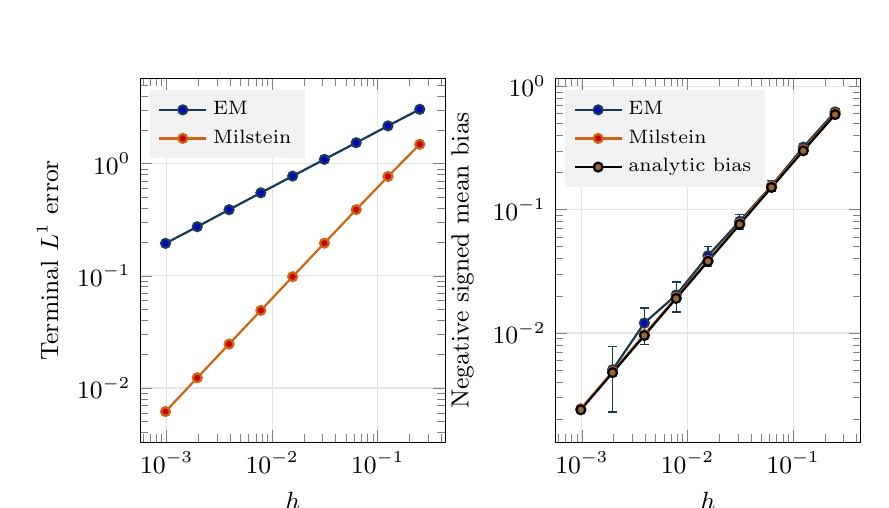
\begin{tikzpicture}
\begin{groupplot}[group style={group size=2 by 1,horizontal sep=1.4cm},width=.45\textwidth,height=6.2cm,legend style={font=\scriptsize},label style={font=\small}]
\nextgroupplot[xmode=log,ymode=log,xlabel={$h$},ylabel={Terminal $L^1$ error},legend pos=north west]
\addplot+[color=navy,mark=*,mark size=1.6pt,thick,error bars/.cd,y dir=both,y explicit] table[x=h,y=v,y error=e] {
h v e
0.25 3.049237871 0.02614903453
0.125 2.172206739 0.01670912847
0.0625 1.537320185 0.0109051874
0.03125 1.091718152 0.007378740046
0.015625 0.7743451398 0.005159110559
0.0078125 0.5494814719 0.003622554849
0.00390625 0.3887253123 0.002542289657
0.001953125 0.2739134636 0.001788696566
0.0009765625 0.1946063729 0.001262415261
};
\addlegendentry{EM}
\addplot+[color=orange,mark=*,mark size=1.6pt,thick,error bars/.cd,y dir=both,y explicit] table[x=h,y=v,y error=e] {
h v e
0.25 1.4880319 0.01205926209
0.125 0.7676999277 0.006240053495
0.0625 0.3893110586 0.003172136946
0.03125 0.1956283052 0.001602660067
0.015625 0.09819580696 0.0008072584469
0.0078125 0.0491675104 0.0004040032449
0.00390625 0.0246252138 0.0002022006167
0.001953125 0.01231668201 0.0001012968403
0.0009765625 0.0061570972 5.067759457e-05
};
\addlegendentry{Milstein}
\nextgroupplot[xmode=log,ymode=log,xlabel={$h$},ylabel={Negative signed mean bias},legend pos=north west]
\addplot+[color=navy,mark=*,mark size=1.6pt,thick,error bars/.cd,y dir=both,y explicit] table[x=h,y=v,y error=e] {
h v e
0.25 0.6205242464 0.0347308512
0.125 0.3209757457 0.02344672045
0.0625 0.1564723285 0.01600079547
0.03125 0.08050976477 0.01113242493
0.015625 0.04232345621 0.007852389177
0.0078125 0.02033829902 0.005549549697
0.00390625 0.01204463101 0.003913119513
0.001953125 0.00504559674 0.002756092909
};
\addlegendentry{EM}
\addplot+[color=orange,mark=*,mark size=1.6pt,thick,error bars/.cd,y dir=both,y explicit] table[x=h,y=v,y error=e] {
h v e
0.25 0.6002320572 0.0159406153
0.125 0.3062088132 0.00824559485
0.0625 0.154964835 0.004187989388
0.03125 0.07742143868 0.002111996405
0.015625 0.03884043293 0.001062291901
0.0078125 0.01944072819 0.0005317634049
0.00390625 0.009738969892 0.0002662177323
0.001953125 0.004866097505 0.0001332875251
0.0009765625 0.002435212914 6.665456997e-05
};
\addlegendentry{Milstein}
\addplot+[color=black,mark=*,mark size=1.6pt,thick] coordinates {(0.25,0.589650816) (0.125,0.299986065) (0.0625,0.151321046) (0.03125,0.0759974291) (0.015625,0.0380835652) (0.0078125,0.019063074) (0.00390625,0.00953686971) (0.001953125,0.00476976928) (0.0009765625,0.0023852184)};
\addlegendentry{analytic bias}
\end{groupplot}
\end{tikzpicture}
\caption{The strong convergence slopes differ noticeably, although both methods have the same first-moment bias in theory. The error bars show the 95\% Monte Carlo intervals. For EM with $N=1024$, the mean-bias interval includes zero, so it is not shown in this log-scale plot. Its signed value is reported in Table \ref{tab:gbm}. The notebook uses a symmetric-log scale to display this interval.}\label{fig:gbm}\end{figure}

The fitted strong convergence slopes, with 95\% joint batch-bootstrap intervals, are 0.4975 [0.4952, 0.4994] for EM and 0.9972 [0.9966, 0.9978] for Milstein. These results are close to the expected rates of 0.5 and 1, respectively. The EM estimate does not have to include exactly 0.5 because the fitting uses a finite range of step sizes. In addition, the bootstrap reflects sampling variability but does not account for truncation errors in the asymptotic expansions. With errors of 0.194606 and 0.006157 at $N=1024$, it is evident that retaining the quadratic variation is decisive for pathwise accuracy.

Regarding weak convergence, the exact bias curve yields a fitted slope of 0.9949. Empirically, the weak-mean slopes are 0.9610 [0.8999, 1.0466] for EM ($N\leq256$) and 0.9948 [0.9938, 0.9957] for Milstein (all levels). The finest EM signed estimate is -0.001819 with a 95\% half-width of 0.001953, which includes zero; therefore, there is no basis to claim a resolved nonzero bias or to blindly fit all EM points. While Milstein's analytic first-moment bias matches EM's, its paired mean estimator exhibits substantially lower variance.

\subsection{Distribution, quantiles and analytic moments}
\begin{figure}[H]\centering
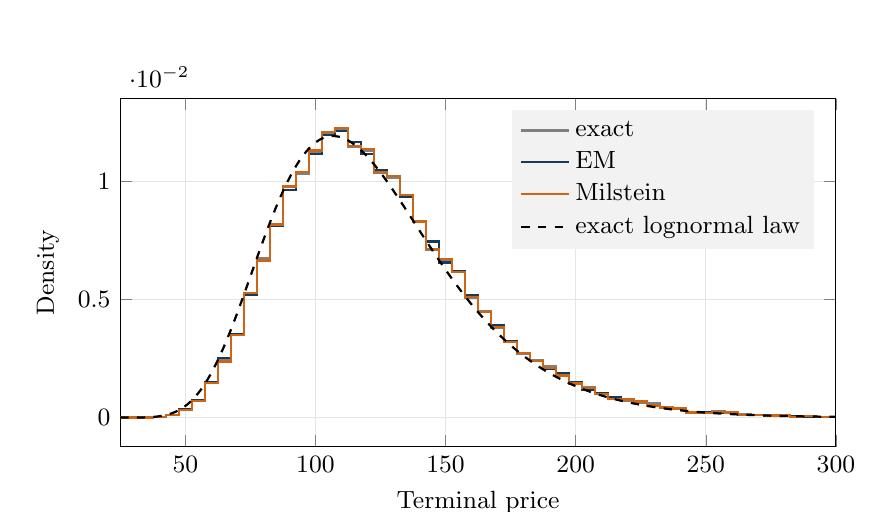
\begin{tikzpicture}
\begin{axis}[xlabel={Terminal price},ylabel={Density},xmin=25,xmax=300,legend pos=north east]
\addplot[color=gray,const plot,thick,no marks] coordinates {(2.5,0) (7.5,0) (12.5,0) (17.5,0) (22.5,0) (27.5,0) (32.5,3.0517578e-06) (37.5,3.3569336e-05) (42.5,0.00010681152) (47.5,0.00032043457) (52.5,0.00075683594) (57.5,0.001473999) (62.5,0.0024810791) (67.5,0.0035308838) (72.5,0.005267334) (77.5,0.0067474365) (82.5,0.0081420898) (87.5,0.0097991943) (92.5,0.010327148) (97.5,0.011236572) (102.5,0.011999512) (107.5,0.012213135) (112.5,0.011447144) (117.5,0.011273193) (122.5,0.010372925) (127.5,0.010125732) (132.5,0.0093994141) (137.5,0.0082855225) (142.5,0.0070953369) (147.5,0.006652832) (152.5,0.0061706543) (157.5,0.0050720215) (162.5,0.0044952393) (167.5,0.0038024902) (172.5,0.0032196045) (177.5,0.0027038574) (182.5,0.0024505615) (187.5,0.0021575928) (192.5,0.0017669678) (197.5,0.0014892578) (202.5,0.0012695313) (207.5,0.0010162354) (212.5,0.0008392334) (217.5,0.00072631836) (222.5,0.00063781738) (227.5,0.00062255859) (232.5,0.0004119873) (237.5,0.00040893555) (242.5,0.00021972656) (247.5,0.00019226074) (252.5,0.00025939941) (257.5,0.0002166748) (262.5,0.00015563965) (267.5,0.00010070801) (272.5,7.6293945e-05) (277.5,9.1552734e-05) (282.5,6.1035156e-05) (287.5,5.1879883e-05) (292.5,3.9672852e-05) (297.5,3.3569336e-05) (302.5,1.8310547e-05) (307.5,2.4414063e-05) (312.5,1.8310547e-05) (317.5,6.1035156e-06) (322.5,1.8310547e-05) (327.5,3.0517578e-06) (332.5,2.746582e-05) (337.5,6.1035156e-06) (342.5,0) (347.5,3.0517578e-06) (352.5,9.1552734e-06) (357.5,6.1035156e-06) (362.5,6.1035156e-06) (367.5,0) (372.5,0) (377.5,0) (382.5,0) (387.5,0) (392.5,0) (397.5,0)};\addlegendentry{exact}
\addplot[color=navy,const plot,thick,no marks] coordinates {(2.5,0) (7.5,0) (12.5,0) (17.5,0) (22.5,0) (27.5,0) (32.5,3.0517578e-06) (37.5,3.9672852e-05) (42.5,0.0001159668) (47.5,0.00034790039) (52.5,0.00075378418) (57.5,0.0015075684) (62.5,0.002532959) (67.5,0.0035522461) (72.5,0.0051879883) (77.5,0.006640625) (82.5,0.0081298828) (87.5,0.0096374512) (92.5,0.010385132) (97.5,0.011141968) (102.5,0.011947632) (107.5,0.012130737) (112.5,0.011642456) (117.5,0.01116333) (122.5,0.010464478) (127.5,0.01022644) (132.5,0.0093292236) (137.5,0.0082611084) (142.5,0.0074462891) (147.5,0.0065643311) (152.5,0.0061981201) (157.5,0.0051971436) (162.5,0.0044769287) (167.5,0.0039031982) (172.5,0.0032348633) (177.5,0.0027313232) (182.5,0.0023803711) (187.5,0.0020751953) (192.5,0.0018737793) (197.5,0.0014831543) (202.5,0.001171875) (207.5,0.0010162354) (212.5,0.00085754395) (217.5,0.00074462891) (222.5,0.00066833496) (227.5,0.00050048828) (232.5,0.00040588379) (237.5,0.00038452148) (242.5,0.00022888184) (247.5,0.00023498535) (252.5,0.00021362305) (257.5,0.00021972656) (262.5,0.00010070801) (267.5,9.765625e-05) (272.5,9.765625e-05) (277.5,7.019043e-05) (282.5,4.8828125e-05) (287.5,3.6621094e-05) (292.5,3.6621094e-05) (297.5,2.4414063e-05) (302.5,2.746582e-05) (307.5,2.1362305e-05) (312.5,3.0517578e-06) (317.5,9.1552734e-06) (322.5,1.8310547e-05) (327.5,1.8310547e-05) (332.5,9.1552734e-06) (337.5,0) (342.5,6.1035156e-06) (347.5,6.1035156e-06) (352.5,9.1552734e-06) (357.5,3.0517578e-06) (362.5,0) (367.5,0) (372.5,0) (377.5,0) (382.5,0) (387.5,0) (392.5,0) (397.5,0)};\addlegendentry{EM}
\addplot[color=orange,const plot,thick,no marks] coordinates {(2.5,0) (7.5,0) (12.5,0) (17.5,0) (22.5,0) (27.5,0) (32.5,0) (37.5,3.0517578e-05) (42.5,0.00010375977) (47.5,0.00030517578) (52.5,0.00071105957) (57.5,0.0014770508) (62.5,0.0023773193) (67.5,0.0034820557) (72.5,0.0052734375) (77.5,0.0066467285) (82.5,0.0081695557) (87.5,0.009777832) (92.5,0.010379028) (97.5,0.011297607) (102.5,0.012088013) (107.5,0.012265015) (112.5,0.011502075) (117.5,0.011364746) (122.5,0.010403442) (127.5,0.010205078) (132.5,0.0094299316) (137.5,0.008291626) (142.5,0.0071166992) (147.5,0.0067199707) (152.5,0.006161499) (157.5,0.0050964355) (162.5,0.0044555664) (167.5,0.0038269043) (172.5,0.0031829834) (177.5,0.0027282715) (182.5,0.0024047852) (187.5,0.0020996094) (192.5,0.0017822266) (197.5,0.0014404297) (202.5,0.001260376) (207.5,0.00099182129) (212.5,0.0008026123) (217.5,0.00076293945) (222.5,0.00067749023) (227.5,0.00050964355) (232.5,0.00043029785) (237.5,0.00038146973) (242.5,0.00021972656) (247.5,0.00018615723) (252.5,0.00025024414) (257.5,0.00021972656) (262.5,0.00012207031) (267.5,0.00010681152) (272.5,8.8500977e-05) (277.5,9.1552734e-05) (282.5,3.9672852e-05) (287.5,5.1879883e-05) (292.5,3.6621094e-05) (297.5,3.3569336e-05) (302.5,2.1362305e-05) (307.5,2.4414063e-05) (312.5,1.2207031e-05) (317.5,3.0517578e-06) (322.5,1.8310547e-05) (327.5,9.1552734e-06) (332.5,2.1362305e-05) (337.5,3.0517578e-06) (342.5,3.0517578e-06) (347.5,3.0517578e-06) (352.5,1.2207031e-05) (357.5,0) (362.5,6.1035156e-06) (367.5,0) (372.5,0) (377.5,0) (382.5,0) (387.5,0) (392.5,0) (397.5,0)};\addlegendentry{Milstein}
\addplot[black,dashed,thick,no marks] coordinates {(25.00000,9.8663144e-08) (26.52778,2.5180967e-07) (28.05556,5.8832867e-07) (29.58333,1.2725459e-06) (31.11111,2.5721267e-06) (32.63889,4.8965245e-06) (34.16667,8.8379263e-06) (35.69444,1.5210618e-05) (37.22222,2.5084064e-05) (38.75000,3.9804976e-05) (40.27778,6.1004297e-05) (41.80556,9.0586171e-05) (43.33333,0.00013069753) (44.86111,0.00018367865) (46.38889,0.00025199659) (47.91667,0.00033816491) (49.44444,0.00044465418) (50.97222,0.00057379803) (52.50000,0.00072770025) (54.02778,0.00090814759) (55.55556,0.0011165327) (57.08333,0.0013537908) (58.61111,0.0016203522) (60.13889,0.0019161131) (61.66667,0.0022404236) (63.19444,0.0025920943) (64.72222,0.0029694185) (66.25000,0.0033702096) (67.77778,0.0037918509) (69.30556,0.0042313543) (70.83333,0.0046854268) (72.36111,0.0051505413) (73.88889,0.005623009) (75.41667,0.0060990516) (76.94444,0.0065748709) (78.47222,0.0070467142) (80.00000,0.0075109344) (81.52778,0.0079640436) (83.05556,0.0084027591) (84.58333,0.0088240422) (86.11111,0.0092251295) (87.63889,0.0096035557) (89.16667,0.0099571702) (90.69444,0.010284146) (92.22222,0.010582983) (93.75000,0.010852504) (95.27778,0.01109185) (96.80556,0.011300465) (98.33333,0.011478082) (99.86111,0.011624706) (101.38889,0.011740589) (102.91667,0.011826216) (104.44444,0.011882274) (105.97222,0.011909634) (107.50000,0.011909324) (109.02778,0.011882508) (110.55556,0.011830463) (112.08333,0.011754557) (113.61111,0.011656229) (115.13889,0.01153697) (116.66667,0.011398305) (118.19444,0.011241776) (119.72222,0.011068929) (121.25000,0.010881298) (122.77778,0.010680397) (124.30556,0.010467708) (125.83333,0.01024467) (127.36111,0.010012676) (128.88889,0.0097730637) (130.41667,0.0095271103) (131.94444,0.0092760308) (133.47222,0.009020974) (135.00000,0.0087630204) (136.52778,0.0085031814) (138.05556,0.0082423985) (139.58333,0.0079815442) (141.11111,0.0077214223) (142.63889,0.0074627695) (144.16667,0.0072062567) (145.69444,0.0069524917) (147.22222,0.0067020208) (148.75000,0.006455332) (150.27778,0.0062128571) (151.80556,0.0059749751) (153.33333,0.0057420146) (154.86111,0.0055142573) (156.38889,0.0052919405) (157.91667,0.0050752603) (159.44444,0.0048643746) (160.97222,0.0046594056) (162.50000,0.0044604432) (164.02778,0.0042675469) (165.55556,0.004080749) (167.08333,0.0039000572) (168.61111,0.0037254562) (170.13889,0.0035569107) (171.66667,0.0033943674) (173.19444,0.0032377566) (174.72222,0.0030869946) (176.25000,0.0029419852) (177.77778,0.0028026212) (179.30556,0.0026687865) (180.83333,0.0025403567) (182.36111,0.002417201) (183.88889,0.0022991834) (185.41667,0.0021861633) (186.94444,0.0020779972) (188.47222,0.001974539) (190.00000,0.001875641) (191.52778,0.0017811548) (193.05556,0.0016909321) (194.58333,0.0016048246) (196.11111,0.0015226855) (197.63889,0.001444369) (199.16667,0.0013697316) (200.69444,0.0012986317) (202.22222,0.0012309304) (203.75000,0.0011664916) (205.27778,0.0011051822) (206.80556,0.0010468723) (208.33333,0.00099143538) (209.86111,0.00093874838) (211.38889,0.00088869183) (212.91667,0.00084114991) (214.44444,0.00079601045) (215.97222,0.00075316501) (217.50000,0.00071250884) (219.02778,0.00067394088) (220.55556,0.00063736378) (222.08333,0.00060268378) (223.61111,0.00056981072) (225.13889,0.00053865799) (226.66667,0.0005091424) (228.19444,0.00048118418) (229.72222,0.00045470685) (231.25000,0.00042963719) (232.77778,0.00040590508) (234.30556,0.00038344348) (235.83333,0.00036218829) (237.36111,0.0003420783) (238.88889,0.00032305505) (240.41667,0.00030506278) (241.94444,0.00028804829) (243.47222,0.0002719609) (245.00000,0.00025675231) (246.52778,0.00024237652) (248.05556,0.00022878975) (249.58333,0.00021595037) (251.11111,0.00020381875) (252.63889,0.00019235724) (254.16667,0.00018153006) (255.69444,0.00017130321) (257.22222,0.00016164443) (258.75000,0.00015252305) (260.27778,0.00014391001) (261.80556,0.00013577772) (263.33333,0.0001281) (264.86111,0.00012085206) (266.38889,0.00011401037) (267.91667,0.00010755266) (269.44444,0.00010145781) (270.97222,9.5705814e-05) (272.50000,9.0277748e-05) (274.02778,8.5155682e-05) (275.55556,8.0322645e-05) (277.08333,7.5762578e-05) (278.61111,7.1460288e-05) (280.13889,6.74014e-05) (281.66667,6.3572322e-05) (283.19444,5.9960196e-05) (284.72222,5.6552868e-05) (286.25000,5.3338848e-05) (287.77778,5.0307275e-05) (289.30556,4.7447887e-05) (290.83333,4.4750984e-05) (292.36111,4.2207405e-05) (293.88889,3.9808493e-05) (295.41667,3.7546073e-05) (296.94444,3.5412424e-05) (298.47222,3.3400255e-05) (300.00000,3.150268e-05)};\addlegendentry{exact lognormal law}
\end{axis}
\end{tikzpicture}
\caption{The histograms compare the price estimates from the different schemes with exact simulation at $N=32$, using a bin width of 5. The analytic lognormal density is also included for comparison. For a clearer view, the plot only shows prices between 25 and 300. However, all 65,536 observations are included in the estimation, with no renormalization. It is worth noting that comparing marginal distributions alone is not enough to assess pathwise errors between coupled simulations.}\label{fig:distribution}\end{figure}

\begin{table}[H]\centering\small
\caption{Quantiles for the center and tails. Even with exact simulation, finite-sample deviations persist.}\label{tab:quant}
\begin{tabular}{rrrrr}\toprule
$p$ & Exact quantile & Exact simulation & EM ($N=32$) & Milstein ($N=32$)\\\midrule
0.01 & 58.106 & 58.032 & 57.644 & 58.280\\
0.05 & 71.287 & 71.348 & 71.312 & 71.565\\
0.50 & 116.766 & 116.740 & 116.877 & 116.724\\
0.95 & 191.259 & 192.508 & 191.771 & 191.907\\
0.99 & 234.645 & 235.721 & 233.999 & 234.685\\
\bottomrule\end{tabular}\end{table}
The theoretical mean is 122.1403, compared with 122.3222 from exact simulation, with a standard error of 0.1473. The sample variance is 1421.9593, which is relatively close to the theoretical value of 1404.9152. We also calculated the average of $(S_T-\mathbb{E}S_T)^2$, obtaining 1421.9707 with a standard error of 10.4649. Since the calculation uses the theoretical mean, this estimator is unbiased for the exact variance. The differences between the simulated and theoretical results are consistent with Monte Carlo sampling variation. Although histograms help us compare the overall distributions, they may not show errors along individual coupled paths. The reported quantiles are also sample-based estimates, so they should not be treated as exact values or formal goodness-of-fit measures.

\subsection{Non-affine reference validation and strong convergence}
The increment sample contains 134,217,728 pairs. For $h_f=1/4096$, the two empirical variances are 0.0002441197 and 0.0002441035, both close to the theoretical value of 0.000244140625. The correlation is -0.6999956, which is also close to the theoretical value of -0.7. All simulated price-factor states stay within the predefined limits, keeping the exponentiated prices strictly positive. The terminal prices range from 25.1046 to 301.2824. These checks suggest that the numerical implementation is working as intended, although they do not establish that the model accurately represents real financial markets.

\begin{table}[H]\centering\small
\caption{Non-affine log EM relative to the $N_r=4096$ EM reference. Signed payoff differences mostly fail to resolve a bias; one isolated significant point is not a weak-rate study. All $\pm$ values are 95\% half-widths.}\label{tab:sv}
\begin{tabular}{rlll}\toprule
$N$ & Strong discrepancy & Call-payoff difference & Bias/SE\\\midrule
8 & $1.25305\pm 0.01224$ & $0.00864\pm 0.01574$ & 1.08\\
16 & $0.89935\pm 0.00846$ & $0.00884\pm 0.01112$ & 1.56\\
32 & $0.63671\pm 0.00593$ & $0.01093\pm 0.00786$ & 2.73\\
64 & $0.44464\pm 0.00413$ & $0.00439\pm 0.00547$ & 1.57\\
128 & $0.31468\pm 0.00289$ & $0.00098\pm 0.00387$ & 0.50\\
256 & $0.22095\pm 0.00202$ & $-0.00004\pm 0.00272$ & -0.03\\
\bottomrule\end{tabular}\end{table}
\begin{figure}[H]\centering
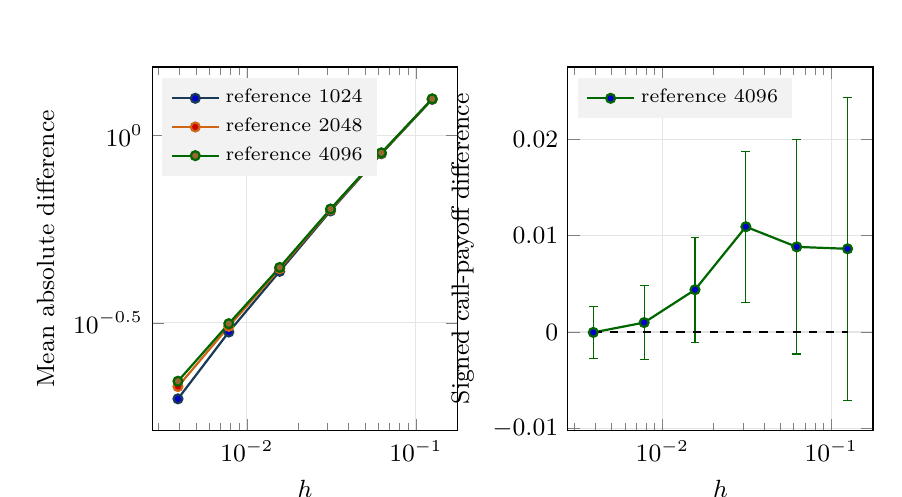
\begin{tikzpicture}
\begin{groupplot}[group style={group size=2 by 1,horizontal sep=1.4cm},width=.45\textwidth,height=6.2cm,legend style={font=\scriptsize},label style={font=\small}]
\nextgroupplot[xmode=log,ymode=log,xlabel={$h$},ylabel={Mean absolute difference},legend pos=north west]
\addplot+[color=navy,mark=*,mark size=1.6pt,thick,error bars/.cd,y dir=both,y explicit] table[x=h,y=v,y error=e] {
h v e
0.125 1.249381887 0.0122097592
0.0625 0.8941932773 0.008415111959
0.03125 0.6292431808 0.005864743423
0.015625 0.4340745774 0.004034408207
0.0078125 0.298887684 0.002756308136
0.00390625 0.1982491285 0.001825646231
};
\addlegendentry{reference 1024}
\addplot+[color=orange,mark=*,mark size=1.6pt,thick,error bars/.cd,y dir=both,y explicit] table[x=h,y=v,y error=e] {
h v e
0.125 1.251866269 0.01222596232
0.0625 0.8970730147 0.008440915422
0.03125 0.6338854215 0.005897910198
0.015625 0.4409285136 0.004094003332
0.0078125 0.3094191845 0.002842289928
0.00390625 0.2137087882 0.001959509049
};
\addlegendentry{reference 2048}
\addplot+[color=green!40!black,mark=*,mark size=1.6pt,thick,error bars/.cd,y dir=both,y explicit] table[x=h,y=v,y error=e] {
h v e
0.125 1.253050938 0.01224051823
0.0625 0.8993490641 0.00846079601
0.03125 0.6367142698 0.005928328294
0.015625 0.4446435137 0.004126943885
0.0078125 0.3146773356 0.00288575396
0.00390625 0.2209472185 0.002021713969
};
\addlegendentry{reference 4096}
\nextgroupplot[xmode=log,xlabel={$h$},ylabel={Signed call-payoff difference},legend pos=north west,scaled y ticks=false,yticklabel style={/pgf/number format/fixed,/pgf/number format/precision=3}]
\addplot+[color=green!40!black,mark=*,mark size=1.6pt,thick,error bars/.cd,y dir=both,y explicit] table[x=h,y=v,y error=e] {
h v e
0.125 0.008643925944 0.01573889383
0.0625 0.008843022846 0.01112185848
0.03125 0.01093488521 0.007856736079
0.015625 0.004391686991 0.005467757518
0.0078125 0.0009813191283 0.00386864306
0.00390625 -4.331509735e-05 0.002715834349
};
\addlegendentry{reference 4096}
\addplot[black,dashed,no marks] coordinates {(0.00390625,0) (0.125,0)};
\end{groupplot}
\end{tikzpicture}
\caption{Nested-grid log EM supports an empirical half-order strong regime, with visible reference sensitivity at small coarse steps. The weak panel is signed and uses a linear vertical scale: intervals crossing zero are displayed rather than converted into spurious log errors. Bars show sampling uncertainty only.}\label{fig:sv}\end{figure}

Using reference sizes $N_r=1024$, $2048$, and $4096$, the estimated convergence rates are 0.5170 [0.5130, 0.5212], 0.5058 [0.5021, 0.5097], and 0.5003 [0.4966, 0.5046], respectively. When the reference size increases from 2048 to 4096, the rate changes by 0.0054, while the strong discrepancy at $N=256$ changes by 3.28\%. Both results meet the operational stability checks. However, the finest coarse-grid point is still affected by the choice of reference, since the shift between references is larger than the Monte Carlo interval. For this reason, we present the empirical rates and discrepancies relative to a finite reference rather than treating them as exact strong errors.

\begin{table}[H]\centering\small
\caption{Reference refinement is a separate source of uncertainty. A small signed weak shift can coexist with a much larger absolute pathwise difference.}\label{tab:ref}
\begin{tabular}{lll}\toprule
Reference pair & Mean absolute price difference & Signed payoff difference\\\midrule
1024-2048 & $0.080764\pm 0.000751$ & $-0.000359\pm 0.001005$\\
2048-4096 & $0.056758\pm 0.000522$ & $0.000308\pm 0.000699$\\
1024-4096 & $0.098672\pm 0.000919$ & $-0.000051\pm 0.001226$\\
\bottomrule\end{tabular}\end{table}
The adjacent-reference strong differences decrease by a ratio 1.423, near $\sqrt2$, consistent with a half-order regime. Their nonzero size matters: the $2048$--$4096$ difference is about 25.7\% of the $N=256$ discrepancy. The triangle inequality implies
\begin{equation}\label{eq:reftriangle}
\left|\E|S_h-S|-\E|S_h-S_r|\right|\le\E|S_r-S|,
\end{equation}
but the right side is unknown. Neither an adjacent-grid difference nor a Richardson extrapolation is a rigorous upper bound without additional assumptions. The reference hierarchy is sufficient for the stated empirical half-order conclusion, not for certifying four-digit exact pathwise error.

\subsection{Weak-payoff uncertainty and a more precise expected payoff}
For the finest reference, the estimated expected payoff is 14.57837 (SE 0.11815), and the estimated value of $\mathbb{E}[S_{N_r}]$ is 105.10376 (SE 0.16795), which is close to the analytical value of 105.12711. However, although this agreement is expected from \eqref{eq:discmart}, it does not tell us how large the weak error in the call payoff is.

In Table \ref{tab:sv}, the confidence intervals for most paired call-payoff differences include zero. Since the results do not show a clear and statistically significant power-law pattern, we do not estimate an empirical weak convergence order for this quantity. Also, because the payoff function has a kink, theorems for smooth test functions cannot be used directly without checking the required regularity conditions. More simulation paths, variance reduction for payoff differences, or a multilevel estimator may help identify a small weak bias.

Using an independent pilot sample, the control coefficient is estimated as $\hat{\beta}=0.6387$, reducing the evaluation-sample variance by a factor of 6.23. On the same subset, the raw payoff estimate is 14.64582 (SE 0.12637), while the controlled estimate is 14.58551 (SE 0.05062, 95\% CI [14.48629, 14.68472]). The control therefore gives a more precise estimate of the fine-grid expected payoff. However, its confidence interval has a half-width of about 0.10, which is much larger than the observed changes between adjacent reference levels. This comparison helps assess the available numerical resolution, but it does not provide a theoretical bound on the continuum price bias.

\subsection{Positivity counterexample}
\begin{table}[H]\centering\small
\caption{Analytic one-step negativity probabilities and observed counts in 200,000 independent updates per row. Stress: $\mu=0.05$, $\sigma=1.5$; baseline: $\mu=0.2$, $\sigma=0.3$.}\label{tab:positive}
\begin{tabular}{lrrrrr}\toprule
Case & $h$ & $p_{EM}$ & EM count & $p_{Mil}$ & Mil. count\\\midrule
baseline & 1.0 & 3.17e-05 & 4 & 0.00000 & 0\\
baseline & 0.5 & 1.08e-07 & 0 & 0.00000 & 0\\
baseline & 0.25 & 1.28e-12 & 0 & 0.00000 & 0\\
baseline & 0.125 & 2.15e-22 & 0 & 0.00000 & 0\\
stress & 1.0 & 0.242 & 48525 & 0.43569 & 87523\\
stress & 0.5 & 0.167 & 33324 & 0.13192 & 26317\\
stress & 0.25 & 0.0885 & 17527 & 0.00000 & 0\\
stress & 0.125 & 0.0289 & 5839 & 0.00000 & 0\\
\bottomrule\end{tabular}\end{table}
Zero observed failures do not prove zero probability: with 200,000 trials, the approximate 95\% upper bound after zero events is $3/M\simeq1.5\times10^{-5}$. The baseline Milstein zero probability follows from the quadratic minimum, not the experiment. At the stressed $h=1$, Milstein actually has a \emph{larger} one-step negativity probability than EM. This falsifies the claim that adding a Milstein correction always improves positivity. All positivity stress parameters are labelled separately from the main convergence benchmark.

\subsection{Extension: preserved moments, limited price advantage}
\begin{figure}[H]\centering
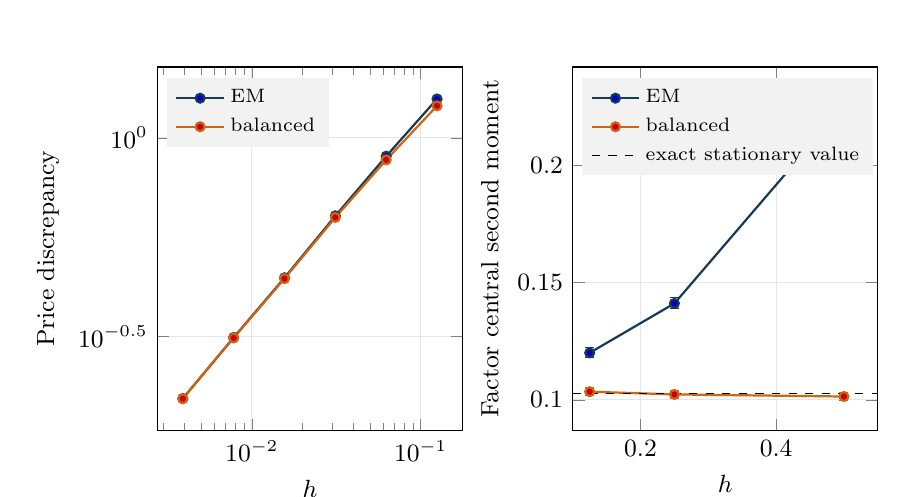
\begin{tikzpicture}
\begin{groupplot}[group style={group size=2 by 1,horizontal sep=1.4cm},width=.45\textwidth,height=6.2cm,legend style={font=\scriptsize},label style={font=\small}]
\nextgroupplot[xmode=log,ymode=log,xlabel={$h$},ylabel={Price discrepancy},legend pos=north west]
\addplot+[color=navy,mark=*,mark size=1.6pt,thick,error bars/.cd,y dir=both,y explicit] table[x=h,y=v,y error=e] {
h v e
0.125 1.253050938 0.01224051823
0.0625 0.8993490641 0.00846079601
0.03125 0.6367142698 0.005928328294
0.015625 0.4446435137 0.004126943885
0.0078125 0.3146773356 0.00288575396
0.00390625 0.2209472185 0.002021713969
};
\addlegendentry{EM}
\addplot+[color=orange,mark=*,mark size=1.6pt,thick,error bars/.cd,y dir=both,y explicit] table[x=h,y=v,y error=e] {
h v e
0.125 1.203975316 0.01171189462
0.0625 0.8803435066 0.008297261573
0.03125 0.6306910963 0.00587211586
0.015625 0.4424733218 0.004108617172
0.0078125 0.3138133364 0.002876010673
0.00390625 0.2206310918 0.002017918777
};
\addlegendentry{balanced}
\nextgroupplot[xlabel={$h$},ylabel={Factor central second moment},legend pos=north west,xmin=0.1,xmax=0.55]
\addplot+[color=navy,mark=*,mark size=1.6pt,thick,error bars/.cd,y dir=both,y explicit] table[x=h,y=v,y error=e] {
h v e
0.5 0.2254169359 0.00362212349
0.25 0.1411427003 0.002356475068
0.125 0.1200590119 0.002108295545
};
\addlegendentry{EM}
\addplot+[color=orange,mark=*,mark size=1.6pt,thick,error bars/.cd,y dir=both,y explicit] table[x=h,y=v,y error=e] {
h v e
0.5 0.1014449172 0.001620561664
0.25 0.1023373636 0.001696980109
0.125 0.1035034417 0.00178757191
};
\addlegendentry{balanced}
\addplot[black,dashed,no marks] coordinates {(0.1,0.102857142857) (0.55,0.102857142857)};\addlegendentry{exact stationary value}
\end{groupplot}
\end{tikzpicture}
\caption{The extension has little effect on fine-grid terminal price error (left), but preserves the exact factor stationary variance across stable coarse steps (right). The latter uses the separate $T=40$, $Y_0=\theta$ stress IVP. The unstable EM $h=1$ row is reported numerically in Table \ref{tab:stress} rather than compressing this axis.}\label{fig:extension}\end{figure}

The balanced scheme exhibits an empirical strong price convergence slope of 0.4872 [0.4835, 0.4908] for $N=8$ to 128 when compared against the EM reference. At $N=8$, the error is 1.20398 for the balanced scheme versus 1.25305 for EM; at $N=256$, these values are 0.22063 and 0.22095, respectively. This minor improvement on the coarse grid does not alter the underlying half-order convergence. Furthermore, at $N=8$, the balanced scheme's payoff difference from the reference is 0.02835 $\pm$ 0.01509, compared to 0.00864 $\pm$ 0.01574 for EM, demonstrating that preserving a factor moment does not necessarily yield a smaller price-payoff bias.

For the factor-only stress experiment, we initialize the factor at $Y_0=\theta=-0.2$ and set $T=40$ with fixed model coefficients. This isolates the exact centered recurrence \eqref{eq:emvar}, distinct from the original one-year IVP, and utilizes 32,768 paths with step sizes $h=1,1/2,1/4,1/8$.

\begin{table}[H]\centering\small
\caption{Factor stress test, $Y_0=\theta$, $T=40$. All uncertainties are nominal 95\% half-widths; the unstable EM $h=1$ interval is unreliable and fails against the exact discrete moment. Stable rows test variance accuracy as well as boundedness.}\label{tab:stress}
\begin{tabular}{lrlll}\toprule
Method & $h$ & $A_h$ & Sample central second moment & Analytic $T=40$ moment\\\midrule
EM & 1.0 & 1.3600 & $11735.9645\pm 8448.8360$ & 228342.9966\\
balanced & 1.0 & 0.1067 & $0.1027\pm 0.0016$ & 0.1029\\
EM & 0.5 & 0.1800 & $0.2254\pm 0.0036$ & 0.2283\\
balanced & 0.5 & 0.2132 & $0.1014\pm 0.0016$ & 0.1029\\
EM & 0.25 & 0.3400 & $0.1411\pm 0.0024$ & 0.1418\\
balanced & 0.25 & 0.4248 & $0.1023\pm 0.0017$ & 0.1029\\
EM & 0.125 & 0.6075 & $0.1201\pm 0.0021$ & 0.1192\\
balanced & 0.125 & 0.6419 & $0.1035\pm 0.0018$ & 0.1029\\
\bottomrule\end{tabular}\end{table}
At $h=1$, standard EM has $A_h=1.36>1$. Starting at $U_0=0$, its exact discrete second moment after $n$ steps is
\begin{equation}\label{eq:stressmean}
v_n=\xi^2h(1+\theta^2)\frac{A_h^n-1}{A_h-1}.
\end{equation}
For $n=40$, the theoretical value is 228343.00, but the simulated sample mean is only 11735.96, which is about 5.1\% of the exact value. The usual normal confidence interval does not contain the theoretical value either. This happens because the expected value is strongly affected by rare paths with very large values. With a finite sample, these extreme paths may not appear often enough, so both the sample mean and the estimated standard error can be misleading. This is not a contradiction of the stability analysis. Instead, it shows a limitation of Monte Carlo estimation in this setting. The deterministic recurrence still confirms that EM is unstable, while the simulation shows that a small estimated error does not always mean the result is accurate. For this reason, we cannot claim reliable 95\% coverage for this stress test.

For the balanced scheme, the variances stay close to 0.102857 across all tested values of $h$, which agrees with Proposition \ref{prop:balanced}. At the coarse step size $h=1/2$, EM gives a stationary variance of 0.228293, more than twice the exact value, although the scheme is still stable. This shows that a stable numerical method does not necessarily reproduce the correct variance or give accurate price estimates. These properties need to be considered separately.

\subsection{Measured cost at a common accuracy target}
\label{sec:cost}
We measure integration cost using the median running time from seven runs after a warm-up, with 8,192 paths and pre-generated Brownian increments. The number of path updates is also reported. The recorded times include the calculations within each solver, memory allocation and any additional stability checks. However, they do not include random number generation, input preparation, library imports, reference solutions, bootstrap calculations, plotting or animation. For the performance comparison, we require the terminal mean-absolute price error to be no greater than 0.5. We use the upper bound of the sampling confidence interval to check this requirement, rather than relying only on the estimated mean error. For each method, we then choose the largest step size that meets this target.

\begin{table}[H]\centering\small
\caption{Measured integration cost for 8,192 paths at a common $0.5$ error ceiling. GBM uses the exact oracle; non-affine errors are relative to $N_r=4096$. The displayed intervals are sampling intervals.}\label{tab:cost}
\begin{tabular}{llrlrr}\toprule
Model & Method & $N$ & Error estimate & Time (ms) & Path updates\\\midrule
GBM & EM & 256 & $0.3887\pm 0.0025$ & 1.4243 & 2,097,152\\
GBM & Milstein & 16 & $0.3893\pm 0.0032$ & 0.1748 & 131,072\\
GBM & exact & 1 & $0$ (exact) & 0.0432 & 8,192\\
Non-affine & EM & 64 & $0.4446\pm 0.0041$ & 6.5389 & 524,288\\
Non-affine & balanced & 64 & $0.4425\pm 0.0041$ & 6.4562 & 524,288\\
\bottomrule\end{tabular}\end{table}
For GBM, EM and Milstein give almost the same error at their selected step sizes, so their computational costs can be compared under similar accuracy requirements. In this experiment, Milstein uses 16 times fewer path updates and runs about 8.15 times faster than EM. Exact terminal simulation is still the best choice for GBM, since it has no discretization error and only needs one Gaussian increment. However, this comparison only applies to terminal values. If the full price path is needed, the methods would have to be compared on the same output grid, which would involve additional computation.

For the non-affine models, both methods use $N=64$ to meet the same reference-error requirement. Their running times are quite similar, and the small differences do not provide enough evidence that one method is generally faster. The measured errors are both around 0.44, but these are errors relative to the numerical reference, not the exact solution. The balanced method therefore does not show a clear computational advantage for the one-year price simulation. Its main benefit is that it preserves the factor moments more accurately, rather than reducing the overall simulation cost.

\subsection{Transient visualisation}
The notebook includes a 65-frame animation showing six non-affine sample paths over one year. Price and instantaneous volatility are displayed in two aligned panels. The paths are generated using a fixed random stream, making the results reproducible. The animation shows how volatility changes with the underlying factor, while prices remain continuous and positive throughout the simulation. However, the animation is mainly used to illustrate the behaviour of the model, rather than to test convergence. Six sample paths are not enough to represent the full distribution. For the statistical results and terminal error analysis, we therefore use a much larger number of independent simulated paths.

\subsection{Guide-compliant rate overlays and cost comparison}
\begin{figure}[H]\centering
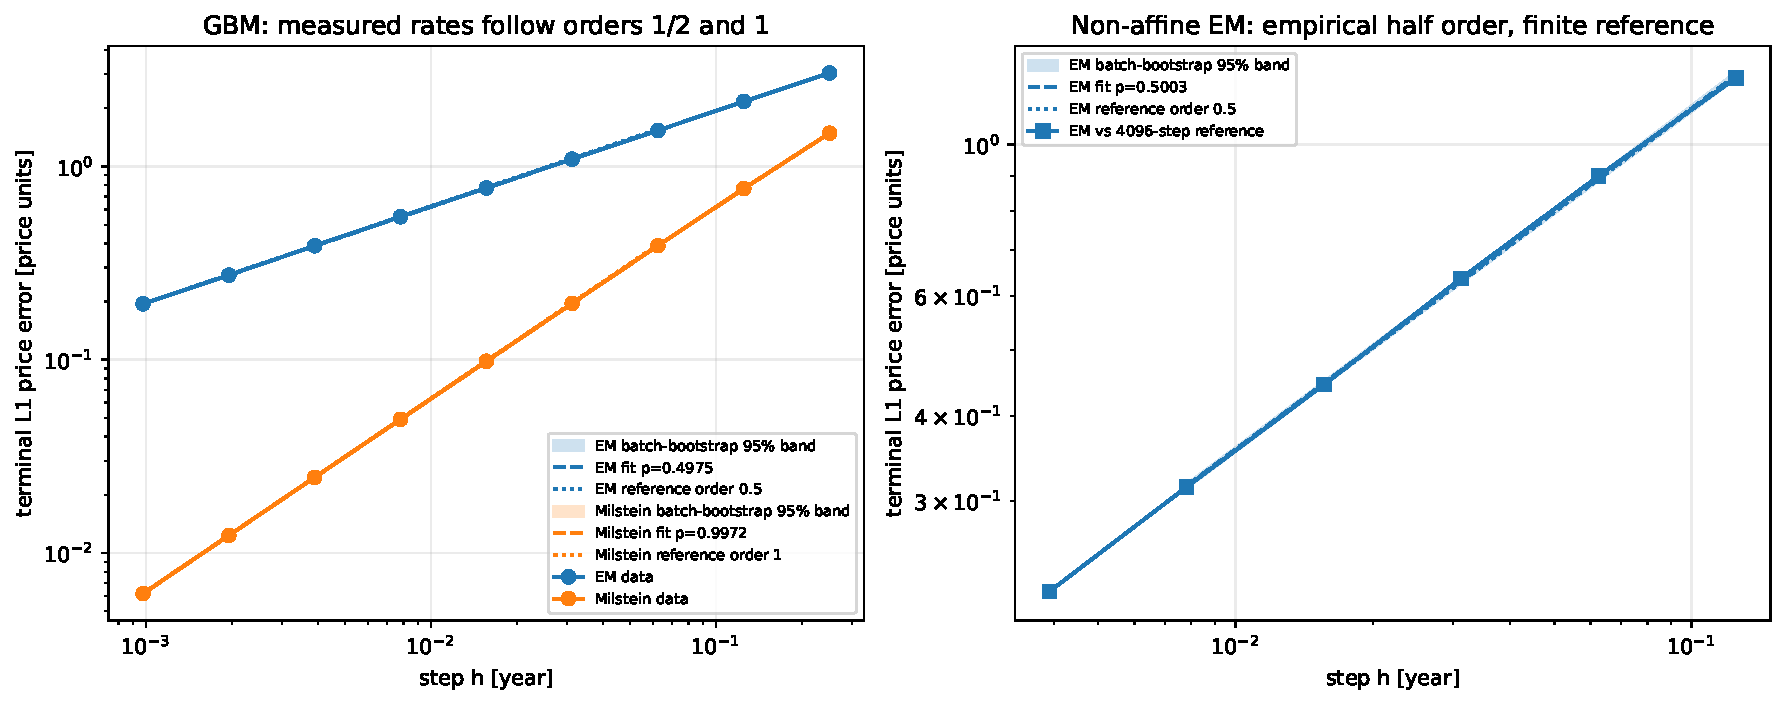
\includegraphics[width=\linewidth]{../../code/project1/outputs/convergence_bands.pdf}
\caption{Strong error against step size in years, with theoretical reference slopes and fitted lines. Shaded regions are pointwise 95\% bootstrap sampling bands from 500 resamples of independent batches; each resample retains its entire vector across grids. GBM uses $N=16,\ldots,1024$ for fitting. The non-affine fit uses $N=8,\ldots,128$ against the 4096-step reference; the displayed $N=256$ point is excluded from the fit. Bands exclude reference and asymptotic-fit bias, and can be visually narrow at this sample size. All values are regenerated by the companion script.}
\end{figure}
\begin{figure}[H]\centering
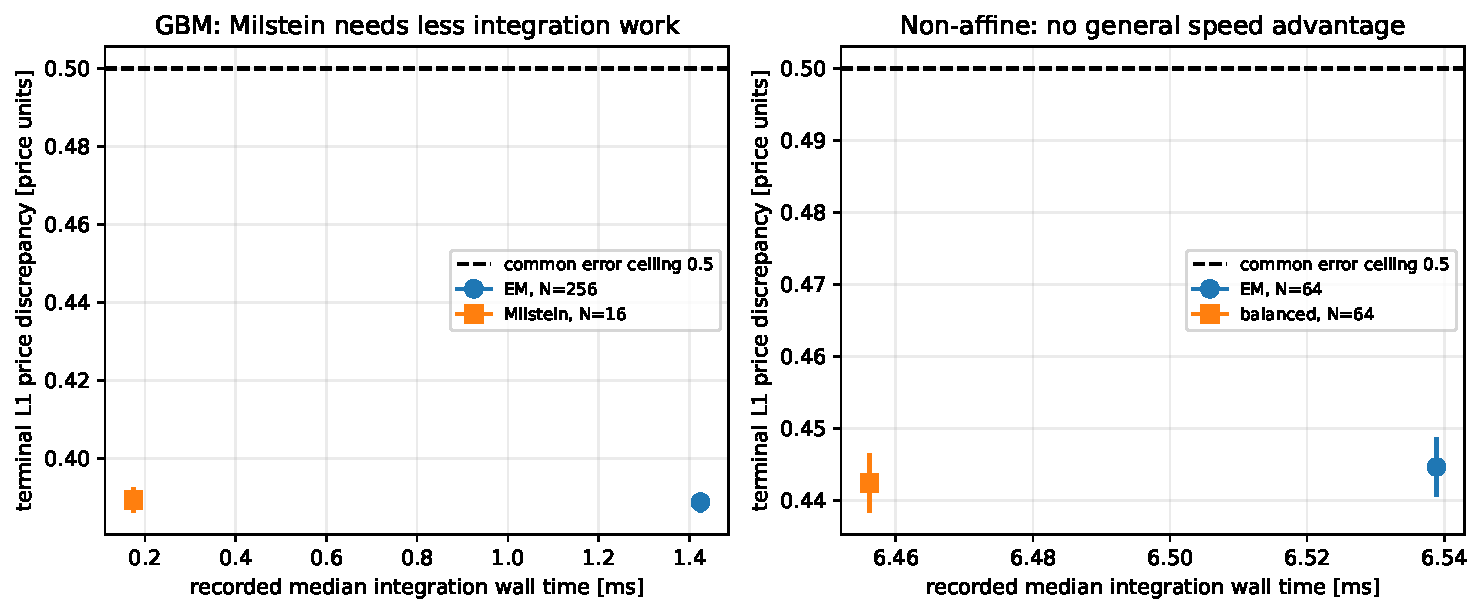
\includegraphics[width=\linewidth]{../../code/project1/outputs/error_vs_cost.pdf}
\caption{Recorded median integration wall time versus achieved terminal $L^1$ discrepancy at the common ceiling 0.5. Vertical intervals are pointwise sampling intervals. Each point is the least costly tested admissible grid, rather than an equal-step comparison. GBM uses the exact pathwise oracle; the non-affine model uses the finite reference. Times are the archived measurements quoted in Table \ref{tab:cost}, on 8192 paths after warm-up, with seven repeats; RNG, setup, reference construction, plotting and bootstrap cost are excluded. Exact GBM has zero time-discretisation error and is discussed separately.}
\end{figure}

\begin{figure}[H]\centering
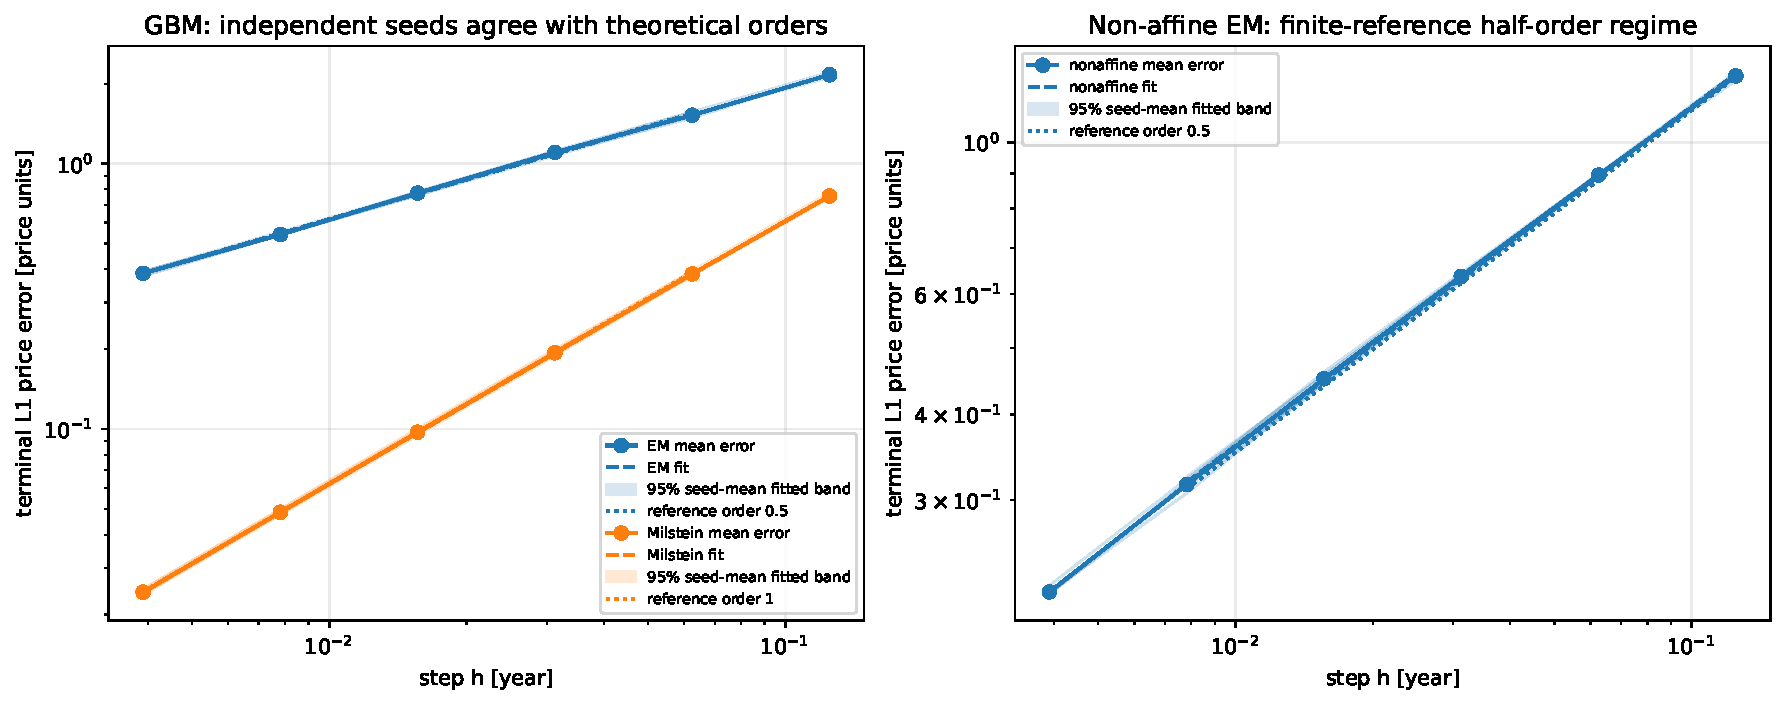
\includegraphics[width=\linewidth]{../../code/project1/outputs/independent_seed_bands.pdf}
\caption{Supplementary whole-experiment repetition over five independent seeds (20261001--20261005), each with 4096 paths and a 4096-step fine grid. Thin lines show seed-specific errors; the fitted mean and an approximate Student-$t$ 95\% band use the spread of the five fitted log-error curves (four degrees of freedom). GBM fits use $N=16,\ldots,256$; non-affine fits use $N=8,\ldots,128$. This checks seed sensitivity separately from the larger main run's batch bootstrap. It is a confidence band for the mean fitted log-error, not a prediction band for a new seed, not simultaneous coverage, and not a bound on reference bias.}
\end{figure}
Five seeds are a limited supplementary replication, not a substitute for a sufficiently large path budget. The exact per-seed errors and slopes are recorded in \texttt{outputs/independent\_seeds.json}; the main inference still relies on the larger experiment, analytic checks and reference refinement.

\section{Limitations, conclusions and practical recommendations}
\label{sec:conclusions}
The GBM experiments show the expected strong convergence orders, together with a first-order mean bias and consistent error distributions. For this model, the exact transition is therefore the most practical option. In the non-affine model, where an exact pathwise solution is not available, the nested refinement results suggest a convergence rate close to one-half. This result should still be treated with some caution, since the estimated errors depend on the numerical reference used. In particular, narrow confidence intervals do not necessarily mean that the true discretization error is known accurately. The weak-payoff differences are also difficult to distinguish from Monte Carlo noise, so the results are not sufficient to estimate a reliable weak convergence order.

For the factor process, we introduced a moment-balanced update and showed that it preserves the exact mean and stationary variance. This removes the second-moment step-size restriction associated with EM for this particular factor. However, the numerical results do not show a clear improvement in the computational cost of one-year price simulations, nor does the method consistently produce smaller payoff biases. The large-step experiment also shows a practical difficulty with Monte Carlo estimation. When a small number of rare paths contribute heavily to a moment, even a relatively large sample may fail to capture their effect. In such cases, the usual confidence intervals can be misleading.

There are several limitations to these results. All parameters are synthetic, and the methods have not been tested using market calibration or hedging experiments. The strong-error analysis considers terminal $L^1$ errors rather than errors over the entire simulated path. In addition, the confidence intervals for the fitted convergence slopes only account for the statistical variation in the regression and do not include possible errors from the assumed asymptotic behaviour or the numerical reference. For the non-affine model, the reference solution is constructed using a refined EM scheme rather than an independent exact method. The exact moment calculations and frozen-factor comparisons provide useful checks, but they cannot fully verify the coupled model. The control variate reduces Monte Carlo variance, although it does not remove the discretization bias in the continuous-time price. The unstable stress test also illustrates why normal confidence intervals should not be trusted when extreme outcomes are poorly represented in the sample. We do not claim methodological novelty, particularly since more advanced methods such as multidimensional Milstein schemes and adaptive Brownian-bridge integrators were not implemented.

In practice, exact GBM simulation is useful for checking an implementation before moving to more complicated models. Simulating the log-price is also preferable when price positivity needs to be maintained. For convergence tests, using the same Brownian paths across different step sizes makes comparisons more informative. Weak-payoff differences should be reported together with their Monte Carlo uncertainty, and the numerical reference should be refined before drawing conclusions about convergence rates. Finally, when accurate financial payoffs are required, sampling error and time-discretization error need to be considered separately. Reporting more decimal places does not, by itself, make a numerical estimate more accurate.

\begin{thebibliography}{99}
\bibitem{brief} Course team. \emph{Project 1 Brief: Numerical Solution of ODE Initial Value Problems}. Supplied course material, Weeks 1--4, 2026. File: \texttt{ODE\_IVP\_Project\_Brief.pdf}.
\bibitem{pack} Course team. \emph{Problem Pack: Five Suggested Directions for the ODE IVP Project}. Direction (4): Financial SDE, GBM benchmark and non-affine volatility. Supplied course material, 2026. File: \texttt{problem\_pack.pdf}.
\bibitem{rubric} Course team. \emph{Assessment Rubrics for PBL Numerical PDEs}. 11 September 2026. Supplied course material. File: \texttt{Numerical\_PDEs\_Assessment\_Rubrics.pdf}.
\bibitem{higham} D. J. Higham. An algorithmic introduction to numerical simulation of stochastic differential equations. \emph{SIAM Review}, 43(3):525--546, 2001. \href{https://doi.org/10.1137/S0036144500378302}{doi:10.1137/S0036144500378302}. Bibliographic existence verified against the publisher and author-affiliated repository; foundational source, not a source of the present experiment's numerical results.
\bibitem{kloeden} P. E. Kloeden and E. Platen. \emph{Numerical Solution of Stochastic Differential Equations}. Springer, 1992. \href{https://doi.org/10.1007/978-3-662-12616-5}{doi:10.1007/978-3-662-12616-5}.
\bibitem{numpy} C. R. Harris et al. Array programming with NumPy. \emph{Nature}, 585:357--362, 2020. \href{https://doi.org/10.1038/s41586-020-2649-2}{doi:10.1038/s41586-020-2649-2}.
\bibitem{scipy} P. Virtanen et al. SciPy 1.0: fundamental algorithms for scientific computing in Python. \emph{Nature Methods}, 17:261--272, 2020. \href{https://doi.org/10.1038/s41592-019-0686-2}{doi:10.1038/s41592-019-0686-2}.
\end{thebibliography}
\clearpage\appendix

\section{Part A -- Team AI Transparency Log}
\label{app:ai}
\textbf{Team D. One collective log for the team.} This report, its mathematical exposition, code and numerical analysis were prepared with AI assistance. Experiments are synthetic simulations. The entries distinguish analytic checks and executed computational evidence from personal review; members must confirm their understanding before signing A4. Routine assistance included array coding, document formatting and rendered-output checks.

\subsection*{A1. AI tools used}
\begingroup\small\setlength{\tabcolsep}{4pt}
\begin{longtable}{@{}p{.22\linewidth}p{.26\linewidth}p{.47\linewidth}@{}}\toprule
Tool & Version / Date & Primary use\\\midrule\endhead
OpenAI Codex & September--October 2026; precise model version not archived & Mathematical exposition, code and experiment preparation, claim checks, report/slide revisions and submission organisation.\\[6pt]
\bottomrule
\end{longtable}\endgroup

\subsection*{A2. Significant AI-assisted claim audits}
Three material claims are audited below; routine edits are summarised above. Original project conversation records are retained separately. Members should correct the entries if their actual work adds or changes evidence.
\begingroup\small\setlength{\tabcolsep}{4pt}
\begin{longtable}{@{}p{.06\linewidth}p{.46\linewidth}p{.43\linewidth}@{}}\toprule
Item & Prompt / claim / assumptions & Risk and possible falsifier\\\midrule\endhead
1 & \textbf{Claim:} scalar Milstein has strong order one on price-space GBM. Assumptions: common Brownian paths, smooth scalar coefficients and finite moments. The task requested the It\^o--Taylor derivation and comparison with EM. & Log-GBM removes the correction, while independent coarse/fine noise invalidates strong comparisons. An incorrect correction or coupled slope far from one would challenge the implementation.\\[10pt]
2 & \textbf{Claim under audit:} the non-affine model has a validated empirical weak order one. Assumptions needed: a resolved reference, observable bias above sampling uncertainty and careful treatment of the nonsmooth payoff. & Absolute noisy sample means can create a spurious slope. Intervals crossing zero or reference-sensitive bias would prevent a rate conclusion.\\[10pt]
3 & \textbf{Claim under audit:} the moment-balanced update is stable and therefore always better. Assumptions: $2\kappa>\xi^2$, fresh Gaussian increments and the specified explicit factor update. Stability here concerns factor second moments. & Stationary-variance stability does not establish exact prices, higher price order or lower cost. Coupled price/cost results can falsify a general superiority claim.\\\bottomrule
\end{longtable}\endgroup

\subsection*{A3. Independent verification and decision}
These checks use analytic special cases and recorded computations, not AI output as its own oracle. Computational checks were executed during the assisted preparation; this does not assert that every member personally ran or independently reviewed them.
\begingroup\small\setlength{\tabcolsep}{4pt}
\begin{longtable}{@{}p{.06\linewidth}p{.46\linewidth}p{.43\linewidth}@{}}\toprule
Item & Independent check and evidence location & Final decision / modification / limitation\\\midrule\endhead
1 & Derive the scalar correction and compare on common paths with the exact exponential. Check transition composition, zero diffusion and the one-step formula. Evidence: Eqs.~\eqref{eq:gbmexact}--\eqref{eq:milstein}, Fig.~\ref{fig:gbm}, \path{code/validation_tests.py}, \path{validation_tests.log}. & Supported for this GBM benchmark: slope 0.9972. Keep the price-space experiment. Do not transfer scalar order one to the joint model; Eq.~\eqref{eq:commutator} shows noncommuting diffusion fields.\\[10pt]
2 & Compare signed coupled payoff differences and their intervals on three reference grids; check the known mean separately. Evidence: Tables~\ref{tab:sv} and \ref{tab:ref}, \path{outputs/results.json}, \path{verification_run.log}. & Reject a validated empirical weak-rate claim at this sample size. Report finite-reference strong convergence and unresolved weak biases. Control variates reduce sampling variance, not reference bias.\\[10pt]
3 & Derive the factor moment recurrence and stationary variance; test the fixed-point identity. Compare stress moments, coupled prices and matched-error cost. Evidence: Proposition~\ref{prop:balanced}, Table~\ref{tab:stress}, Fig.~\ref{fig:extension}, Table~\ref{tab:cost}, \path{code/validation_tests.py}. & Accept the precise factor mean/variance stability claim; reject universal price or speed superiority. The stressed EM interval is unreliable when rare-event tails are undersampled.\\\bottomrule
\end{longtable}\endgroup

\subsection*{A4. Intellectual ownership declaration}
Each member identifies their actual contribution and signs their own row. Signing affirms that they can explain and modify the team-owned numerical methods, justify the claims, and state assumptions and tests at trusted library interfaces without AI during the viva. Personal signatures and understanding are not inferred here.

\textbf{Team-owned artefacts:} directly implemented updates, Brownian coupling, error estimators, factor-moment proofs, tests and interpretation. \textbf{Trusted dependencies:} NumPy array arithmetic and random generation; SciPy sigmoid/normal functions; Matplotlib plotting; Pillow GIF export. Codex assistance is disclosed in A1 and is not a numerical-library interface.
\begingroup\small\setlength{\tabcolsep}{4pt}
\begin{longtable}{@{}p{.18\linewidth}p{.17\linewidth}p{.32\linewidth}p{.27\linewidth}@{}}\toprule
Name & Signature / date & Team-owned artefact / contribution & Trusted dependency and interface\\\midrule\endhead
Xihan Chen\newline 2360253 & \rule{.9\linewidth}{.3pt}\newline Date: 2026-10-11 & Report Secs.~1 and 5; EM/Milstein convergence slides: error definitions, uncertainty and reproducibility. & NumPy random-number generation: independent paths and shared Brownian increments across grid levels; documented variance and correlation checks.\\[18pt]
Bowen Duan\newline 2362211 & \rule{.9\linewidth}{.3pt}\newline Date: 2026-10-11 & Non-affine SDE explanation; joint EM/Milstein distinction; nested Brownian grids and control-variate interpretation (Secs.~2.3, 3.4--3.5, 5.1, 5.4). & NumPy Gaussian increments require variance $h$ and correlation $\rho$; SciPy \texttt{expit} gives bounded logistic volatility. Relevant checks are in A3; personal verification must be confirmed before signing.\\[18pt]
Shuyu Teng\newline 2362204 & \rule{.9\linewidth}{.3pt}\newline Date: 2026-10-11 & Numerical scheme derivation, stability and moment-balanced scheme analysis (Secs.~3, 4). & Dependencies: NumPy, SciPy. Assumptions on Brownian increments; stability and positivity numerical checks.\\[18pt]
Conghao Liang\newline 2362212 & \rule{.9\linewidth}{.3pt}\newline Date: 2026-10-11 & Project manager: scope, presentation review, revision decisions and submission organisation. & Team dependency boundaries listed above; personally confirm understanding before signing.\\[18pt]\bottomrule
\end{longtable}\endgroup

\section{Part B -- Individual Contribution Statements (ICS)}
\label{app:ics}
\textbf{Four individual records for Team D, one page per member.} All four statements are included with member names, student IDs and signatures. Each member should confirm the final wording of their own statement.
\clearpage
\subsection*{Individual Contribution Statement -- Project 1 (ODE IVP) -- Xihan Chen}
\textbf{Team:} D \quad \textbf{Name:} Xihan Chen \quad \textbf{Student ID:} 2360253

\textbf{Role this project:} Report Writing and Convergence Analysis Presentation

\textbf{The specific things I did this project:}
\begin{enumerate}[leftmargin=*]
\item I wrote the research background and objectives, explaining why geometric Brownian motion provides an exact benchmark and why the non-affine volatility model requires numerical references. I clarified the scope of the investigation and its focus on reliable numerical simulation.
\item I prepared the presentation content on strong and weak convergence for Euler-Maruyama and Milstein. I explained shared Brownian paths, terminal mean absolute errors, signed mean biases and convergence-rate estimation. I organised the material from definitions to calculations and results, including the influence of Monte Carlo uncertainty.
\item I documented the experimental design and reproducibility procedures, including nested Brownian grids, confidence intervals, bootstrap slope estimates and reference-refinement checks. I explained the separation of discretisation error from sampling uncertainty, the purpose of control variates, and the reported random seeds, implementation choices and validation checks.
\end{enumerate}

\textbf{What I would do differently:}\newline I would simplify the convergence explanations earlier and use one numerical example to connect the formulas with the graphs.

\textbf{Anything I should have asked for help with earlier:}\newline I should have clarified strong versus weak error and the interpretation of confidence intervals earlier.

\textbf{Evidence / Part A cross-reference:}\newline The submitted presentation and report, and the recorded discussion of convergence definitions and calculations. Related AI audits: Part A, A2-A3, items 1-2. This statement describes writing and presentation work, not personal execution of the reported code tests.

\vspace{8mm}\textbf{Signature:} \rule{5cm}{.3pt} \qquad \textbf{Date:} 2026-10-11
\clearpage
\subsection*{Individual Contribution Statement -- Project 1 (ODE IVP) -- Bowen Duan}
\textbf{Team:} D \quad \textbf{Name:} Bowen Duan \quad \textbf{Student ID:} 2362211

\textbf{Role this project:} Mathematical Theory

\textbf{The specific things I did this project:}
\begin{enumerate}[leftmargin=*]
\item I explained the non-affine stochastic-volatility model prescribed in the Problem Pack, including the log-price equation, mean-reverting factor, bounded logistic volatility and correlated Brownian drivers. This explanation corresponds to report Section 2.3.
\item I explained the use of Euler--Maruyama for the joint system and why the scalar Milstein formula cannot be transferred directly. The noncommuting diffusion fields require cross terms and iterated stochastic integrals for a full multidimensional Milstein method. I also explained nested Brownian grids for coupled comparisons (Sections 3.4--3.5 and 5.1).
\item I explained the control-variate construction for the expected call payoff, including the known stock-price mean, the separate pilot sample and the evaluation sample. I clarified that variance reduction improves sampling precision but does not remove time-discretisation bias (Sections 5.4 and 6.4).
\end{enumerate}

\textbf{What I would do differently:}\newline I would reduce unnecessary theorems and organise the explanation around the model, numerical method and interpretation of results.

\textbf{Anything I should have asked for help with earlier:}\newline I should have asked earlier for a clearer explanation of multidimensional noise and the distinction between sampling variance and discretisation bias.

\textbf{Evidence / Part A cross-reference:}\newline Evidence: the report sections listed above and the supplied personal statement. Related AI audits: Part A, A2--A3, items 1--2. My contribution here concerns theoretical explanation; I do not claim personal execution of the code tests.

\vspace{8mm}\textbf{Signature:} \rule{5cm}{.3pt} \qquad \textbf{Date:} 2026-10-11
\clearpage
\subsection*{Individual Contribution Statement -- Project 1 (ODE IVP) -- Shuyu Teng}
\textbf{Team:} D \quad \textbf{Name:} Shuyu Teng \quad \textbf{Student ID:} 2362204

\textbf{Role this project:} Report Writing and Numerical Defects Presentation

\textbf{The specific things I did this project:}
\begin{enumerate}[leftmargin=*]
\item I did the writing work of section 3, which is about numerical methods and convergence concepts. And I completed the derivation for scalar Milstein correction term, exact weak-error formula for GBM and correlated Brownian increment construction. I also explained why scalar Milstein can't be directly applied to the two dimensional non-affine stochastic-volatility model through diffusion commutator argument in the paragraph.
\item I did the writing work of section 4, which is about the stability, positivity and a derived extension. I derived one-step negativity-probability formulas for both EM and Milstein method. I inferred that the second-moment recurrence of the stochastic-volatility factor using standard EM and built up the moment-balanced factor scheme together for the exact conditional mean and stationary variance in period.
\item I performed mathematical sanity-checks linking theory to numerical experiments and I checked that the log-price EM martingale property and find out limitations within the report text. In the presentation I was responsible for discussing the comparison between EM, Milstein sample distributions and the true logarithmic normal distribution and the positivity-negative price issue, which related to what I responsible for in the report.
\end{enumerate}

\textbf{What I would do differently:}\newline I would separate theoretical derivations and numerical sanity-check work earlier.

\textbf{Anything I should have asked for help with earlier:}\newline I should agree with teammates on the symbols variables at very beginning cause this saves time and effort comparing to change these to the same in the end.

\textbf{Evidence / Part A cross-reference:}\newline Report source \path{financial_sde_report.tex} (Section 3, Section 4) and corresponding presentation materials. Related AI audits: Part A, A2-A3, items 1-3.

\vspace{8mm}\textbf{Signature:} \rule{5cm}{.3pt} \qquad \textbf{Date:} 2026-10-11
\clearpage
\subsection*{Individual Contribution Statement -- Project 1 (ODE IVP) -- Conghao Liang}
\textbf{Team:} D \quad \textbf{Name:} Conghao Liang \quad \textbf{Student ID:} 2362212

\textbf{Role this project:} Project Manager

\textbf{The specific things I did this project:}
\begin{enumerate}[leftmargin=*]
\item I set the project scope around the GBM benchmark and non-affine volatility model. I supplied the course materials and requested checks against the rubric, report template and submission requirements. I organised the report, code package and presentation as separate deliverables and arranged suggested responsibilities for the four members.
\item I reviewed the presentation and directed revisions to \path{financial_sde_presentation.tex} and \path{financial_sde_speaker_script.md}. I requested explicit It\^o and EM/Milstein formulas, clearer strong and weak convergence calculations, distribution comparisons and negative-price conditions. I also identified a gap in the transition to stochastic volatility and requested explanations connected to the model equations. I adjusted slide layout, content and length through successive reviews.
\item I used OpenAI Codex to assist with mathematical exposition, code generation, experiments and document preparation. I requested limitations, verification evidence and an AI Transparency Log. My contribution was scope management, critical questioning and revision decisions; I do not claim independent implementation of \texttt{gbm} or \texttt{sv}, or personal execution of the recorded tests.
\end{enumerate}

\textbf{What I would do differently:} I would establish the report structure and presentation timing earlier, and record review decisions alongside revisions.

\textbf{Anything I should have asked for help with earlier:} I should have clarified convergence definitions and the distinction between analytic results and simulation estimates earlier.

\textbf{AI audit cross-reference:} Report Appendix A, especially Audit 1 (scalar Milstein) and Audit 2 (weak-rate interpretation). The assistance used was OpenAI Codex in the recorded project conversation.

\textbf{Evidence:} Recorded requests and revisions in the project conversation; \path{financial_sde_presentation.tex}, \path{financial_sde_speaker_script.md}, and the final submission package. No Git commit history is claimed.

\textbf{Signature:} \rule{5cm}{.3pt} \qquad \textbf{Date:} 2026-10-11

{\small Prepared from the recorded project conversation. The member must review this statement, confirm or adjust the reflections and sign personally. No personal signature or Git history is inferred.}
\clearpage
\section{Reproducibility and submission instructions}
\label{app:reproduce}
Extract \texttt{project1\_code.zip}; from its \texttt{code\_package} folder run:
\begin{lstlisting}[language={},numbers=none]
python -m pip install -r requirements.txt
python code/validation_tests.py
python code/run_all.py
\end{lstlisting}
Use Python 3.10 or newer. The full run regenerates JSON tables, all static figures, rate bands, cost figures and the path animation. Paths are anchored to the script's folder, not to a particular computer. No market data or network access is required after dependency installation. The README states seeds, batch sizes, dependency bounds, timing exclusions and how archived and fresh outputs differ.

The fresh submission run used Python 3.12.14, NumPy 2.5.3, SciPy 1.18.1, Matplotlib 3.11.2 and Pillow 12.3.0; the executable log is retained. The 12 integrated checks and eight separate analytic tests passed. The deliberately unstable stress case remains a reported negative result. A standard confidence interval is not asserted to have reliable coverage when the relevant tail is undersampled.

In the editable source ZIP, compile the root-level \texttt{project1\_report.tex} using Tectonic or pdfLaTeX twice. Keep its \texttt{code\_package} folder alongside the root-level main source. The local working copy uses a \texttt{sources} directory with relative paths adjusted accordingly. It embeds the main Python script using \texttt{filecontents*}, so compile in a dedicated directory. Helper/test listings and the supplementary figures are relative external files included in the bundle. The bibliography is inline. The submission consists of report PDF, code ZIP and the 17-page slides PDF; the source bundle is supplied separately for editing, not as a replacement for those three files.

\textbf{Declarations.} All data are synthetic, with no participants or private market datasets. No funding or conflict information was supplied; members must confirm their own declarations. AI use is disclosed in Appendix \ref{app:ai}. Names, contributions, signatures and historical evidence must be completed from authentic team records.

\clearpage
\section{Presentation and viva preparation}
\label{app:viva}
The companion PDF preserves the approved 17 slides. Suggested ten-minute allocation: slides 1--3 (1.5 minutes, motivation and exact solution); slides 4--5 (1 minute, retained It\^o--Taylor terms); slides 6--9 (2 minutes, strong/weak calculations and results); slides 10--11 (1 minute, distributions); slides 12--13 (1 minute, positivity); slides 14--15 (1.5 minutes, non-affine model and multidimensional limitation); slides 16--17 (2 minutes, coupled references and factor/control-variate extension). Rehearsal is required to check this estimate. Detailed proofs and additional experiments belong in this report. At the user's direction, separate closing and backup slides were removed; the presenter should close slide 17 verbally with the main result and one limitation.

\textbf{Cross-role questions everyone should answer.}
(1) Why must fine Brownian increments be summed rather than regenerated? Because strong error compares approximations on the same driving trajectory.
(2) Why can both methods have the same weak mean bias but different strong orders? The correction is centred but captures a pathwise fluctuation.
(3) Why is a correct mean insufficient for the non-affine solver? Log EM preserves that moment at every step size.
(4) Why is the finest reference not exact? It is still an EM discretisation, and adjacent-reference changes are nonzero.
(5) Why not use scalar Milstein twice? The diffusion fields do not commute.
(6) What did the new scheme actually improve? The factor mean and stationary variance/stability, not a proved price order or general speed advantage.
(7) Why did the stress interval fail? Rare events dominated the expectation, so the sample variance itself was unreliable.
(8) What cost was excluded? RNG, reference construction, setup and plotting; the timed object was integration on fixed input arrays.

\clearpage
\section{Complete executable computational source}
\label{app:code}
The first listing is the main executable source supplied in \texttt{code/run\_all.py}. The code ZIP also supplies its importable kernels, the supplementary visualisation helper and the analytic checks. All are listed below so that the numerical and validation procedures are reviewable.
\lstinputlisting{run_all.py}
\subsection*{Importable kernels used by the special-case tests}
\lstinputlisting{../../code/project1/code/kernels.py}
\subsection*{Supplementary rate and cost figures}
\lstinputlisting{../../code/project1/code/submission_figures.py}
\subsection*{Independent whole-experiment seed repetitions}
\lstinputlisting{../../code/project1/code/repeat_seeds.py}
\subsection*{Independent analytic checks}
\lstinputlisting{../../code/project1/code/validation_tests.py}
\end{document}
